\documentclass[11pt]{article}
%\usepackage[utf8]{inputenc}
\usepackage[english]{babel}
 
%\usepackage{multicol}
\usepackage{amsmath}
\usepackage{amssymb}
\usepackage{amsfonts}
\makeatletter
\def\amsbb{\use@mathgroup \M@U \symAMSb}
\makeatother
\usepackage{bbold}
\usepackage{amsthm}
\usepackage{tabularx}
\usepackage[]{hyperref}
\usepackage[doublespacing]{setspace}
\usepackage{graphicx}
\usepackage{subcaption}
%\graphicspath{ {Figures/} }
\usepackage[a4paper,left=1in,top=1in,right=1in,bottom=1in,nohead]{geometry}

%\topmargin 0.0cm
%\leftmargin -2.5 cm
%\rightmargin -2.5 cm
%\oddsidemargin 0.2cm
%\textwidth 16cm 
%\textheight 21cm
%\footskip 1.0cm

\newtheorem{prop}{Proposition}
\theoremstyle{definition}
\newtheorem{defn}{Definition}

\DeclareMathAlphabet{\pazocal}{OMS}{zplm}{m}{n}
\DeclareMathOperator*{\argmin}{arg\,min}
\date{}

\begin{document}
\title{A Framework for Telescope Schedulers: With Applications to the Large Synoptic Survey Telescope}
\author{Elahesadat Naghib, Peter Yoachim, Robert J. Vanderbei, Andrew J. Connolly, Lynne Jones}

%\affil[a]{Princeton University}
%\affil[b]{Princeton University}
%s\affil[c]{University of Washington}
\maketitle
%\begin{multicols}{2}


\begin{abstract}

Feature-Based telescope scheduler is an automated, proposal-free decision making algorithm that offers \textit{controllability} of the behavior, \textit{adjustability} of the mission, and quick \textit{recoverability} from interruptions for large ground-based telescopes. It is easy to understand, implement and troubleshoot because of its coherent mathematical representation. Accordingly it can be modified by the astronomy community for context-dependent adjustments. This paper presents a raw version of the Feature-Based scheduler, with minimal manual tailoring, to demonstrate its potential and flexibility as a foundation for large ground-based telescope schedulers that can later be adjusted for other instruments. In addition, an adjusted version of the Feature-Based scheduler for LSST is introduced and compared to previous LSST scheduler simulations.
\end{abstract}

\begin{table*}[h]\resizebox{\textwidth}{!}{%
\begin{tabular}{l  l }
\multicolumn{2}{c}{\textbf{Key terms and notations}} \\ \hline
fields & fixed partitions of the sky that can be covered in a single visit, \\
$N_{f}$ & total number of the fields,\\
$t$& Greenwich Mean Time, in Modified Julian Date,\\ 
$\tau_s(t)$ ($\tau_e(t)$)& beginning (end) of the night that $t$ lies in,\\
$\tau_{rise\text{(}set\text{)}}(i,f,t)$ & rising (setting) time of field-filter $(i,f)$ above (below) the acceptable airmass horizon at current night,\\
$\tau_n(i,f,t)$& time of the last visit of field-filter $(i,f)$ before $\tau_s(t)$,\\
$id(t)$ & ID number of the field that is visited at $t$,\\
$ft(t)$& camera's filter at $t$,\\
$n(i,f,t)$ & total number of the visits of field-filter $(i,f)$ before $t$,\\
$slew(i,j)$& slew time from field $i$ to field $j$ in seconds,\\
$settling(i,j)$& mechanical settling time after slewing from field $i$ to field $j$,\\
$\Delta t_{f}$& time needed to change filter, a constant value about 2 minutes,\\
$t_{dome}(i)$& time needed to move the dome to make field $i$ visible to the telescope,\\
$ha(i,t)$ & hour angle of the center of field $i$ at $t$ in hours, $-12 \leq ha(i,t) \leq 12$,\\
$am(i,t)$ & airmass of the center of field $i$ at $t$,\\
$br(i,t)$ & brightness of the sky at the center of field $i$ at $t$,\\
$\sigma(i,t)$ & seeing of the sky at the center of field $i$ at $t$,\\
$K(i,f, t)$ & atmospheric extinction coefficient\\
$W_1, W_2$ & given constant time window within which a revisit is valid, \\
$I_{survey}$ & set of all fields in $survey \in \{WFD,DD,NES,GP,SCP\}$ ,\\ \hline
\end{tabular}}
\end{table*}

\section{Introduction}
The Large Synoptic Survey telescope (LSST), the top national ground-based telescope of the NASA 2010 Decadal Review, with the largest digital camera that has ever been built for astronomy, offers an optical throughput of more than 50 times greater than the best current value \cite{tyson2002large}. Scientific investigations with LSST range from the solar system objects to the edge of the optical universe. 
Even with the powerful engine that enables this telescope to slew fast, satisfying all of the desirables and constraints is a challenging problem. Specifically, the LSST's science-driven mission (explained in \cite{ivezic2008large}) is highly constrained and contains competing objectives that are vastly different in nature, due to the different nature of the scientific expectations. In this paper, we propose a framework to formulate the problem of scheduling for large ground-based telescopes such as LSST then introduce a scheduler based on the proposed model.\\
First generation schedulers for astronomical purposes were developed for space missions to automate their operation due to their inaccessibility, in addition to optimize their scientific productivity. ROSAT mission's scheduler in 1990 \cite{nowakovski1999using},  Spike \cite{johnston1994spike}, Hubble Telescope's scheduler in 1994, and HSTS \cite{muscettola1995automating} in 1995 are amongst pioneering developments on algorithmic scheduling of observations in the space missions.\\
Despite the similarity of the ultimate goal in the missions of space telescopes and ground-based telescopes, determining factors for the purpose of scheduling are fundamentally different. While space-based telescopes are required to respect kinematical and dynamical constraints, earth's atmosphere is the main challenge in the scheduling of ground-based telescopes. The former is predictable and efficiently computable, while the later involves both inherent uncertainties, and uncertainties due to the computational limitations.\\
Earlier algorithmic approaches to the scheduling of ground-based telescopes are heavily based on hand-crafted observation proposals that are generally tested only for feasibility, but not necessarily for optimality. For instance,  Keck Telescope, 1993 \cite{nelson1985design} is run 100\% based on proposals, and Hobby-Eberly Telescope 1997 \cite{shetrone2007ten} has a semi-manual scheduling scheme.\\
Later, appearance of more expensive ground-based instruments with complex missions made it impossible to rely on hand-crafted proposals solely. Need for more efficient use of the instrument's time lead to the development of decision making algorithms for accessible facilities as well, and mainly to optimize their science output. For instance, scheduler of the Liverpool robotic telescope was designed in 1997 to automate and optimize the procedure of time allocation to chunks of scripted schedules. The time allocation strategy was preferred to the scheduling at the single visit level which is referred to as optimum scheduling by the authors of \cite{steele1997control}. The reason for choosing the time allocation scheme instead of optimum scheduling is stated to be the lack of recoverability of the latter choice in case of an interruption, because it potentially leads to excessive computational cost to reevaluate the sequence once it is interrupted. In this paper, we show that scheduling in the single visit level can be quickly recoverable in a memoryless framework, thus the optimality can be preserved.\\
Still, in spite of the reliability of the fully automatic scheduling technologies, there are modern, expensive telescopes such as SALT, 2005 \cite{brink2008salt}, and ALMA 2013 \cite{wootten2003atacama} that are run based only on traditional hand-crafted proposals. ALMA in particular, requires a highly regulated structure for proposals that potentially leads to suboptimality as discussed in \cite{alexander2017enabling}, where the authors suggest a number of corrections for the scheduling regulations to provide adaptivity to time-sensitive observations. However, even with occasional corrections, a verbal policy does not provide verifiable adjustability to the change of mission, as the operation of the telescope reveals newfound scientific desirables.\\
It seems that refusing to adopt the cutting-edge technology of fully automated scheduling for modern astronomical instruments is mainly due to the rooted notion of the observation proposals that perfectly served the scheduling of smaller, slower, and single-mission instruments in the past. This also could be a result of astronomer's lack of trust toward the performance of the decision making machines in every levels of the scheduling. The LSST community, however, in addition to a proposal-based scheduler, introduced in \cite{delgado2016lsst}, have been supporting the design and implementation of proposal-free decision machines, such as Feature-Based scheduler, first introduced in \cite{naghib2016feature}, as well as a variant of the fast marching army cadence by D. Rothchild et al. (2018, in preparation) that explore the possibility of a new generation of the schedulers for fast, multi-mission, big-data collecting instruments.\\
In Section~\ref{sec_SM}, first we explain the choice of Markovian framework for the Feature-Based scheduler, and in Sections~\ref{sec_Markov} and~\ref{sec_Markov_approx} we provide the mathematical details of the scheduler model in that framework. Section~\ref{sec_opt} presents two approaches for the optimization of the model's parameters. Sections~\ref{sec_lsst_problem} and~\ref{sec_lsst_opt} demonstrate the application of the Feature-Based scheduler on LSST which is then followed by a comparison between a modified version of the Feature-Based scheduler and LSST's current official scheduler in Section~\ref{sec_comp}. Finally, Section~\ref{sec_conclusion} presents our concluding remarks.

\section{Scheduling framework}\label{sec_SM}
To run a multi-mission, ground-based telescope such as LSST, the scheduler has to offer \textit{controllability}, \textit{adjustability}, and \textit{recoverability}.
\begin{itemize}
\item \textbf{Controllability}: The high-level mission objectives have to show sufficient variabilities with the variation of the model parameters. Otherwise, either the choice of the input  information is irrelevant to the mission objectives, or the structure of the scheduler is degenerate. Controllability is necessary for a scheduler to be optimizable by the choice of the model parameters. 
\item \textbf{Adjustability}: For a complex, multi-objective mission it is common that the high-level objectives are required to be adjusted in the middle of the operational period. Adjustments take place according to updates of scientific desirables, or based on a feedback provided by the study of the system's performance. Regardless of the reason for the adjustments, a scheduler must offer a systematic flexibility to be adjusted with a reasonable computational cost, and preferably no expert intervention. Hand-tuned scheduling strategies and verbal policies for instance, are not fully adjustable.
\item \textbf{Recoverability}: The presence of unpredictable factors in the operation of ground-based telescopes are due to the natural stochastic processes (such as the weather), and complexity of the mechanical facility. Unscheduled downtimes and filter breakdowns are examples of the many unpredictable survey interruptions. On the other hand, there are inherently predictable interruptions, such as maintenance downtimes, and cable winding that also, due to the complexity of the mechanical system, are not computationally affordable and/or valuable to keep track of. Therefore, they are considered as stochastic variables as well. Given all the stochastic factors, a scheduler is required to be able to quickly output an alternative decision, once a previously unpredictable variable took a value, as well as occurrence of an interruption, for which the scheduler is expected to return to its normal behavior, as quickly as possible, once the interruption is over. A pre-calculated sequence of decisions for instance, lacks the recoverability attribute. Also, strategies with heavy look-back or look-ahead are not fast recoverables. 
\end{itemize}
The Feature-Based scheduler is designed based on a Markovian model in which the flow of the input information, the decision procedure and it's relationship to the mission's objective are coherently expressed. Therefore, controllability of the scheduler is well-defined and verifiable. And it is adjustable, because of the Markovian structure that offers an explicit derivation of the design elements from high-level objectives, and finally is swiftly recoverable due to the inherent memorylessness of the Markovian decision process that for a decision at any time, only requires the current state of the system.

\subsection{Markovian representation}\label{sec_Markov}
\begin{defn}
Let $X_{(.)}$ be a stochastic process for which $X_i$ represents the state of the system at $t_i$, and $\pazocal{S}$ be the set of all possible states that the system can take. Let $\mathbb{P}(X_i)$, be the probability distribution of $X_i$ on $\pazocal{S}$, then $X(.)$ is a Markovian process, if and only if, it satisfies the following \textit{memorylessness} property,
\begin{equation*}
\forall i ~~~~~~~\mathbb{P}(X_{{i+1}} | X_{i}) = \mathbb{P}(X_{{i+1}} | X_{i}, X_{{i-1}},\dots, X_{0}),
\end{equation*}
where $\mathbb{P}(X_{{i+1}} | X_{i})$ is the conditional probability distribution of the system's state at $t_{i+1}$ given it's state at $t_i$, and $\mathbb{P}(X_{{i+1}} | X_{i}, X_{{i-1}},\dots, X_{0})$ is the conditional probability distribution of the system's state at $t_{i+1}$, given all of the states that the system has been in until $t_i$.
\end{defn}
Memorylessness property asserts that the system's next state only depends on its current state and is independent of its earlier history. This property, is in fact, the main reason for choosing a Markovian framework for the scheduler. Accordingly, in the modeling level it requires a state description such that the behavior of the system can be determined by the current state of the system. And consequently, in the scheduling level, a decision can be made based only on the current state of the system.
\begin{defn}
Let $<\pazocal{S},\pazocal{A}, P_a(.,.), R_a(.,.), \gamma>$, be a \textit{Markovian Decision Process (MDP)}, where $\pazocal{A}$ is the set of actions, and $P_a(x, y)$ transition probability from state $x$ to $y$ which is equal to $\mathbb{P}(X_{i+1}=y | X_i=x, a)$, conditional probability of transition from state $x$ to state $y$ given action $a \in  \pazocal{A}$. Similarly the transition reward is denoted by $R_a(x,y)$, and $\gamma \in (0,1]$ is the discount factor.
\end{defn}
\begin{defn}
Action $a_{i} \in \pazocal{A}$ is \textit{admissible} for $<\pazocal{S},\pazocal{A}, P_a(.,.), R_a(.,.), \gamma>$, if it is,
\begin{enumerate}
\item feasible: It is possible to be taken at $t_i$,
\item progressively measurable: only dependent on the current state of the system $X_i$.
\end{enumerate}
\end{defn}
To control the system is to take an action at all decision steps $t_i$. For a Markovian control, the actions are required to be dependent only on the current state to preserve the memorylessness property of the closed-loop system, that's why we require the action to be progressively measurable. Notice that the decision steps $\{ t_i: 0 \leq i \leq N, t^N  =T\}$, from $t_0$, start of the process, to $T$, time horizon of the process, are not necessarily uniformly spaced, and are determined by the time that each transition takes. 
\begin{defn}
A \textit{deterministic policy} $\pi : \pazocal{S} \rightarrow \pazocal{A}_i$, is a mapping from $\pazocal{S}$ to the set of all admissible actions at $t_i$, denoted by $\pazocal{A}_i$. 
\end{defn}
A policy provides a time invariant control law that for all possible $x_i \in \pazocal{S}$ suggests an admissible action for transition to the next state, which automates the control of the system.
\begin{defn}
\textit{A deterministic optimal policy} $\pi$ is a solution to the following optimization problem,
\begin{equation}\label{equ_opt1}
\begin{aligned}
& \underset{\pi}{\text{maximize}}
& & E_{\pi}[\sum_{i = 0}^N \gamma^i R_{\pi(X_{i-1})}(X_{i-1}, X_{i}) | x_0],
\end{aligned}
\end{equation}
where $x_0$ is a given initial state.
\end{defn}
In other words, a deterministic optimal policy maximizes the expected discounted sum of the rewards. By discounting the later rewards versus earlier rewards through $\gamma$, we tune the priority of the overall gain versus instant gains.
\begin{prop} \label{prop_main}
For the Markove decision process of $<\pazocal{S},\pazocal{A}, P_a(.,.), R_a(.,.), \gamma>$, there exists a deterministic optimal policy, and it can be written as follows, 
\begin{equation}\label{equ_opt_pol}
\pi^*= \argmin_{a_{i} \in \pazocal{A}_i} E[\Phi(X_{{i+1}}) | a_{i}],
\end{equation}
where $\Phi: \pazocal{S} \rightarrow \rm I\!R$ is a function.
\end{prop}
\begin{proof}
Consider a function $C_{\pi}: \pazocal{S} \rightarrow \rm I\!R$, defined as follows,
\begin{equation*}
\begin{aligned}
C_{\pi}(x_{i}) &= -E_{\pi}[ \sum_{i\leq j}^N \gamma^{i - j} R_{\pi(X_j)}(X_{j}, X_{{j+1}}) |x_{i}]\\
& = - E_{\pi}[R_{\pi(x_i)}(x_{i}, X_{{i+1}}) | x_{i}] - \gamma E_{\pi}[ \sum_{ i+1 \leq j}^N \gamma^{j-(i+1)} R_{\pi(X_j)}(X_{j}, X_{j+1}) | x_{i}].\\
\end{aligned}
\end{equation*}
Then by applying the the law of total expectation on the second term,
\begin{equation*}
\begin{aligned}
C_{\pi}(x_{{i}}) &= - E_{\pi}[R_{\pi(x_i)}(x_{i}, X_{{i+1}}) | x_{i}] - \gamma E_{\pi}[ E_{\pi}[ \sum_{ i+1 \leq j}^N R_{\pi(X_j)}(X_{j}, X_{{j+1}}) |X_{{i+1}}]| x_{i}]\\
&=  - E_{\pi}[R_{\pi(x_i)}(x_{i}, X_{{i+1}}) | x_{i}] - \gamma E_{\pi}[ C_{\pi}({X_{{i+1}}})| x_{i}],
\end{aligned}
\end{equation*}
and by assuming a finite state space,
\begin{equation*}
C_{\pi}(x_{{i}}) =  - E_{\pi}[R_{\pi(x_i)}(x_{i}, X_{{i+1}}) | x_{i}]  - \gamma \sum_{x_{i+1} \in \pazocal{S}} \mathbb P(x_{i+1}|\pi(x_i), x_{i}, x_{i-1},\dots, x_{0}) C_{\pi}({x_{{i+1}}}).\\
\end{equation*}
Then by the Markov property,
\begin{equation*}
\begin{aligned}
C_{\pi}(x_{i}) &=  - E_{\pi}[R_{\pi(x_i)}(x_{i}, X_{{i+1}}) | x_{i}] - \gamma \sum_{x_{i+1} \in \pazocal{S}} P_{\pi(x_{i})}(x_{i},x_{i+1}) C_{\pi}({x_{{i+1}}}),\\
\end{aligned}
\end{equation*}
where, $P_{\pi(x_{i})}(x_{i},x_{i+1}) $ is the transition probability from $x_i$ to $x_{i+1}$ under the action of $\pi(x_i)$. 
Now, let $C^*(x_{i}) = \min_{\pi} C_{\pi}(x_{{i}})$ then,
\begin{equation}\label{equ_proof1}
\begin{aligned}
C^{*}(x_{{i}}) &=  ~~~~~~~ \min_{\pi}(- E_{\pi}[R_{\pi(x_i)}(x_{i}, X_{{i+1}}) | x_{i}] - \gamma \sum_{x_{i+1} \in \pazocal{S}} P_{\pi(x_{i})}(x_{i},x_{i+1}) C_{\pi}({x_{{i+1}}}))\\
& =  \min_{\{\pi(x_{i}), \pi(x_{{i+1}}),\dots \}}(- E_{\pi}[R_{\pi(x_i)}(x_{i}, X_{{i+1}}) | x_{i}] - \gamma \sum_{x_{i+1} \in \pazocal{S}} P_{\pi(x_{i})}(x_{i},x_{i+1}) C_{\pi}({x_{{i+1}}}))\\
& = ~~~~~~~ \min_{\pi(x_{i})} (- E_{\pi}[R_{\pi(x_i)}(x_{i}, X_{{i+1}}) | x_{i}] - \min_{\{\pi(x_{i+1}), \pi(x_{{i+2}}),\dots \}} \gamma \sum_{x_{i+1} \in \pazocal{S}} P_{\pi(x_{i})}(x_{i+1},x_{i}) C^{\pi}({x_{{i+1}}})).\\
\end{aligned}
\end{equation}
Note that both of the one step reward $R_{\pi(x_i)}(x_{i}, X_{{i+1}})$ and transition probability $P_{\pi(x_{i})}(x_{i}, X_{{i+1}})$ depend only on $\pi(x_{i})$ which is the action taken at $t_i$. 
For the next time step, one can construct a $\hat {C}$ function such that, 
\begin{equation*}
\hat C(x_{{i+1}}) = \min_{\pi(x_{{i+1}})} \min_{\pi} C^{\pi} ({x_{i+1}}).
\end{equation*}
then, 
\begin{equation*}
\begin{aligned}
\sum_{x_{i+1} \in \pazocal{S}} P_{\pi(x_{i})}(x_{i},x_{i+1}) \min_{\{\pi(x_{i+1}), \pi(x_{{i+2}}),\dots \}} C^{\pi}({x_{{i+1}}})&= \sum_{x_{i+1} \in \pazocal{S}} P_{\pi(x_{i})}(x_{i},x_{i+1})  \hat C ({x_{{i+1}}} )\\
& \geq \min_{\pi} \sum_{x_{i+1} \in \pazocal{S}} P_{\pi(x_{i})}(x_{i+1},x_{i}) C^{\pi}({x_{{i+1}}})).
\end{aligned}
\end{equation*}
On the other hand, 
\begin{equation*}
\sum_{x_{i+1} \in \pazocal{S}} P_{\pi(x_{i})}(x_{i},x_{i+1}) \min_{\{\pi(x_{i+1}), \pi(x_{{i+2}}),\dots \}} C^{\pi}({x_{{i+1}}}) \leq \min_{\pi} \sum_{x_{i+1} \in \pazocal{S}} P_{\pi(x_{i})}(x_{i},x_{i+1}) C^{\pi}({x_{{i+1}}})).
\end{equation*}
Therefore,
\begin{equation*}
 \min_{\pi} \sum_{x_{i+1} \in \pazocal{S}} P_{\pi(x_{i})}(x_{i},x_{i+1}) C^{\pi}({x_{{i+1}}}))=\sum_{x_{i+1} \in \pazocal{S}} P_{\pi(x_{i})}(x_{i},x_{i+1}) \min_{\{\pi(x_{i+1}), \pi(x_{{i+2}}),\dots \}} C^{\pi}({x_{{i+1}}}).
\end{equation*}
By substituting the second term of the right hand side of Equation (\ref{equ_proof1}) with the right hand side of the above equation,
\begin{equation*}
\begin{aligned}
C^{*}(x_{{i}}) &= \min_{\pi(x_{i})} (- E_{\pi}[R_{\pi(x_i)}(x_{i}, X_{{i+1}}) | x_{i}] -\gamma \sum_{x_{i+1} \in \pazocal{S}} P_{\pi(x_i)}(x_{i},x_{i+1}) \min_{\pi} C^{\pi}({x_{{i+1}}}))\\
&= \min_{\pi(x_{i})} (- E_{\pi}[R_{\pi(x_i)}(x_{i}, X_{{i+1}}) | x_{i}] -\gamma \sum_{x_{i+1} \in \pazocal{S}} P_{\pi(x_i)}(x_{i},x_{i+1}) C^*({x_{{i+1}}})),\\
\end{aligned}
\end{equation*}
where the last equalities follow from the definition of $C^*$, and is in the form of the optimal bellman equation, for which a solution exists [Bellman 1957], and $C^*(x_0) = \min{C^\pi(x_0)}$ attains the optimal value, by construction of $C^\pi(x_0)$ that is equal to $- E[\sum_{0}^N R_{\pi(x_i)}(x_{{i}}, x_{i+1}) | x_0]$.\\
Given a $C^*$, an optimal policy can be simply evaluated,
\begin{equation}\label{equ_proof2}
\begin{aligned}
\pi^*(x_{i}) & = \argmin_{a_{i} \in \pazocal{A}_i} (- E_{\pi}[R_{a_i}(x_{{i}}, X_{i+1}) | x_{i}] -\gamma \sum_{x_{i+1} \in \pazocal{S}} P_{a_i}(x_{i},x_{i+1})C^*({x_{{i+1}}}))\\
& = \argmin_{a_{i} \in \pazocal{A}_i} (- E_{\pi}[R_{a_i}(x_{{i}}, X_{i+1}) - \gamma C^*({X_{{i+1}}}))| x_{i}].\\
\end{aligned}
\end{equation}
Finally, define,
\begin{equation}\label{equ_phi}
\Phi(X_{{i+1}}) := R_{a_i}(x_{{i}}, X_{i+1}) - \gamma C^*({X_{{i+1}}})),
\end{equation}
 and substitute in Equation (\ref{equ_proof2}) in order to obtain Equation (\ref{equ_opt_pol}).
\end{proof}
For the telescope scheduler we require the policy to be deterministic, because the simulations have to be repeatable for comparison and evaluation purposes, however it can be shown that the deterministic optimal policy is not only optimal amongst deterministic policies, but also is optimal amongst stochastic policies. Therefore the choice of deterministic policy does not harm the optimality of the control. \\
As a result of Proposition~\ref{prop_main}, the solution space of the optimization problem (\ref{equ_opt1}), can be reduced from search over the set of policies to search over $\Phi$ functions.

\subsection{Markovian approximation}\label{sec_Markov_approx}
For a decision that is inherently time dependent, such as scheduling an observation, only a maximal definition of the system's state yields a perfect Markovian Process, in which case, state-space includes all of the possible decision sequences. In particular, LSST requires a sequence of about 1000 decisions at each night. Therefore, storing all possible scenarios requires a state space of size $N_{f}^{1000}$, that clearly is neither tractable nor storable in a realistic memory. In order to overcome the curse of dimensionality, we have designed a set of   \textit{features} to summarize the most important information required for the scheduling. Thus, the system of telescope-environment is only an approximated Markovian Process, once its state-space is replaced by a \textit{feature-space}. \\
On the other hand, despite the reduction of the search space from the mapping space to the function space, made possible by Proposition~\ref{prop_main}, Problem (\ref{equ_opt1}) is still an infinite dimensional optimization problem because its variable is a function. To be able to numerically compute the $\Phi$ function, we propose a parametrized function approximation for $\Phi(x_{i})$,
\begin{equation*}
 \tilde{\Phi}_{\theta}({x}_{i}) := \sum_{j=1}^m \theta_j \Phi_j(x_{i}),
\end{equation*}
where $\theta$ is the vector of variables that characterize $\tilde{\Phi}(.)$, and, $\Phi_i(x_i)$'s are \textit{basis functions} that are designed to modify the features in order to incorporate the astronomical observational knowledge into the decision maker's structure. With this approximation, the space of search is reduced from the space of functions to a finite dimensional vector space. This approximation substitutes the original optimal policy (\ref{equ_opt_pol}) with the following approximate policy,
\begin{equation}\label{equ_approx_pol}
\begin{aligned}
\tilde{\pi}_{\theta}^*(x_{i})& = \argmin_{a_{i}} E[ \tilde{\Phi}_{\theta^*}(X_{i+1}) | a_{i}]\\
& =  \argmin_{a_{i}} \sum_{j=1}^k \theta^*_j E[\Phi_j(X_{i+1}) | a_{i}],\\
\end{aligned}
\end{equation}
where $\theta^*$ is a solution to the following optimization problem,
\begin{equation}\label{equ_opt3}
\begin{aligned}
& \underset{\theta}{\text{maximize}}
& & E_{\pi_{\theta}}[\sum_{i=0}^N \gamma^i R_{\pi_{\theta} (X_{i-1})}(X_{{i-1}}, X_{i}) | x_0],
\end{aligned}
\end{equation}
in which policy $\pi$ is fully determined by $\theta$.

\section{Scheduler optimization}\label{sec_opt}
Given the approximated optimal policy in Equation (\ref{equ_approx_pol}), the only remaining fundamental step to have a scheduler, is to find $\theta^*$ by solving Problem (\ref{equ_opt3}). The following two sections describe two different approaches to find a $\theta^*$. The first approach requires a specific class of the high-level mission objective function, and is faster. The second approach is applicable for all types of the high-level mission objective functions, however requires more computational resources. 

\subsection{Reinforcement Learning}
Assume that there exists a well-defined notion of the instant reward for each state transition, then by the definition of $\Phi(x_{{i}})$ given in Equation (\ref{equ_phi}) one has,
\begin{equation} \label{equ_learning1}
\begin{aligned}
\Phi(x_{i}) &= - R_{\pi^*(x_{i-1})}(x_{i-1},x_i) - \gamma C^*({x_{i}})\\
&= - R_{\pi^*(x_{i-1})}(x_{i-1},x_i) - \gamma E_{\pi^*}[R_{\pi^*(x_{i})}(x_{i},X_{i+1})  +\gamma C^*({X_{{i+1}}})|x_i]\\
&= - R_{\pi^*(x_{i-1})}(x_{i-1},x_i)  + \gamma E_{\pi^*}[\Phi(X_{{i+1}})|x_i].\\
\end{aligned}
\end{equation}
Equation (\ref{equ_learning1}) is valid when the system is operated by the optimal policy, $\pi^*$. Accordingly, for the parametrized $\Phi$ function, we require that,
\begin{equation} \label{equ_learning2}
\begin{aligned}
\tilde \Phi_{\theta^*}(x_{i}) &=  - R_{\pi_{\theta^*}(x_{i-1})}(x_{i-1},x_i)  + \gamma E_{\pi_{\theta^*}}[\tilde \Phi_{\theta^*}(X_{{i+1}})|x_i].\\
\end{aligned}
\end{equation}
The main idea to find the best approximate $\tilde {\Phi}(.)$ is to start the process of the decision making with an arbitrary set of variables, $\theta^0$, and make the decisions according to Policy (\ref{equ_approx_pol}) with the associated $\tilde \Phi_{\theta}(.)$, then update the variables in each decision step, so that $\Phi$'s linear approximation gradually respects Equation (\ref{equ_learning2}) for all $i \in \{j: t_0 \leq t^j \leq T\}$.
Note that at $t_i$, after the transition from $x_{{i-1}}$ to $x_{{i}}$ we have the value of $R_{\pi_{\theta^i}}(x_{i-1},x_i) $ already evaluated in the decision making procedure, and  $\Phi_{\theta^i}(x_{i})$ can be approximated by $E_{\pi_{\theta^i}}[ \Phi_{\theta^i}(x_{i})]$ which is also evaluated in the decision making process, where $\theta^i$ is the last version of the optimization variables at $t_i$. Using the desired value given in Equation (\ref{equ_learning2}), the update is as follows,
\begin{equation}\label{equ_updatePHI}
\begin{aligned}
\tilde \Phi_{\theta^{i+1}}(x_{{i}}) = (1-\alpha) \tilde \Phi_{\theta^{i}}(x_{{i}})+ \alpha  ( \gamma  E_{\pi_{\theta^i}}[\tilde \Phi_{\theta^{i}}(x_{{i+1}})|\pi_{\theta^{i}}(x_{{i}})] -R_{\pi_{\theta^i}}(x_{i-1},x_i) ),
\end{aligned}
\end{equation}
in which, $0<\alpha<1$ is the learning rate. The first term in the right hand side of the equation is the latest approximated value of the $\tilde \Phi$ function associated with $\theta^i$ with $(1-\alpha)$ amount of contribution, and the second term is the value of $\tilde \Phi$ function according to Equation (\ref{equ_learning2}) with $\alpha$ amount of contribution. Clearly for smaller $\alpha$'s this update imposes smaller adjustments. Accordingly, updates of the variables $\theta_j,~~j=1,\dots, k$ can be expressed as follows,
\begin{equation} \label{equ_TD_update}
\begin{aligned}
\theta_j^{i+1} &= \theta_j^{i} + \Big( \tilde \Phi_{\theta^{i+1}}(x_{{i}})  - \tilde \Phi_{\theta^{i}}(x_{{i}}) \Big)\Phi_j(x_{i})\\
& = \theta_j^{i} + \alpha \Big(-\Phi_{\theta^{i}}(x_{{i}}) + \gamma  E_{\pi_{\theta^i}}[\tilde \Phi_{\theta^{i}}(X_{{i+1}})|x_{{i}}] -R_{\pi}(x_{i-1},x_i)  \Big)\Phi_j(x_{i}).
\end{aligned}
\end{equation}
This Learning method is called \textit{Temporal-Difference} (TD) learning with function approximation \cite{tsitsiklis1997analysis}. Variants of this reinforcement learning method have been successfully applied to real-life problems such as training of a backgammon player \cite{tesauro1995temporal}.
Note that to be able to use the TD reinforcement learning method, it is necessary to have a well-behaved notion of the reward that reflects the instant gain of any decision at all of the decision steps. Moreover, the discounted sum of the instant rewards has to reflect the objective of the mission. For instance, in the LSST scheduling problem, after each visit, the negative of the slew time, is a well-defined instant reward that reflects how time-efficiently the telescope is being used, however it does not reflect all aspects of the mission's objective such as, efficiency of the same night revisits (explained in Section~\ref{sec_lsst_problem}), for which there is no equivalent instant reward. For this reason, we also implemented a global optimizer for the LSST scheduler that does not require a notion of the instant reward and directly optimizes the mission's objective function over a limited  episode of the simulated scheduling. 

\subsection{Global Optimization}\label{sec_gopt}
In the absence of a well-defined instant reward, instead of solving problem~\ref{equ_opt3}, The following problem can be solved:
\begin{equation}%\label{equ_opt4}
\begin{aligned}
& \underset{\theta}{\text{maximize}}
& & U_{\pi_{\theta}}(x_i,x_{i+1}, \dots, x_{j}),
\end{aligned}
\end{equation}
where $U_{\pi_{\theta}}(x_i,x_{i+1}, \dots, x_{j})$ is a utility function that measures the performance of the scheduler on a simulated episode of the operation from $t_i$ to $t_j$ by policy $\pi_{\theta}$. In this approach, a general $U(.)$, can not be explicitly expressed as a function of $\theta$, therefore a global optimizer that can maximize a black-box function is required. We used the $e$DE metaheuristic evolutionary optimizer \cite{naghib2016entropic} which is an an adaptive version of the Differential Evolution (DE) algorithm (\cite{storn1997differential}). DE is generally one of the most efficient evolutionary algorithms and the $e$DE variant uses a notion of entropy to automatically preserve the diversity of the candidate solutions. As a result, in contrast with DE, it does not require the user to choose any tuning parameters for the algorithm, which is the most time-consuming task in using an evolutionary optimizer. In addition, $e$DE, similar to any other evolutionary algorithm is highly parallelizable, and the computational time can be almost linearly decreased with respect to the number of computational cores.  

\section{Problem of Scheduling for LSST}\label{sec_lsst_problem}
The LSST mission is to uniformly scan the visible sky within 5 different regions (Figure~\ref{fig_proposals}), each with certain science-driven desirables and constraints.\\
\begin{figure}[h!]
\begin{center}
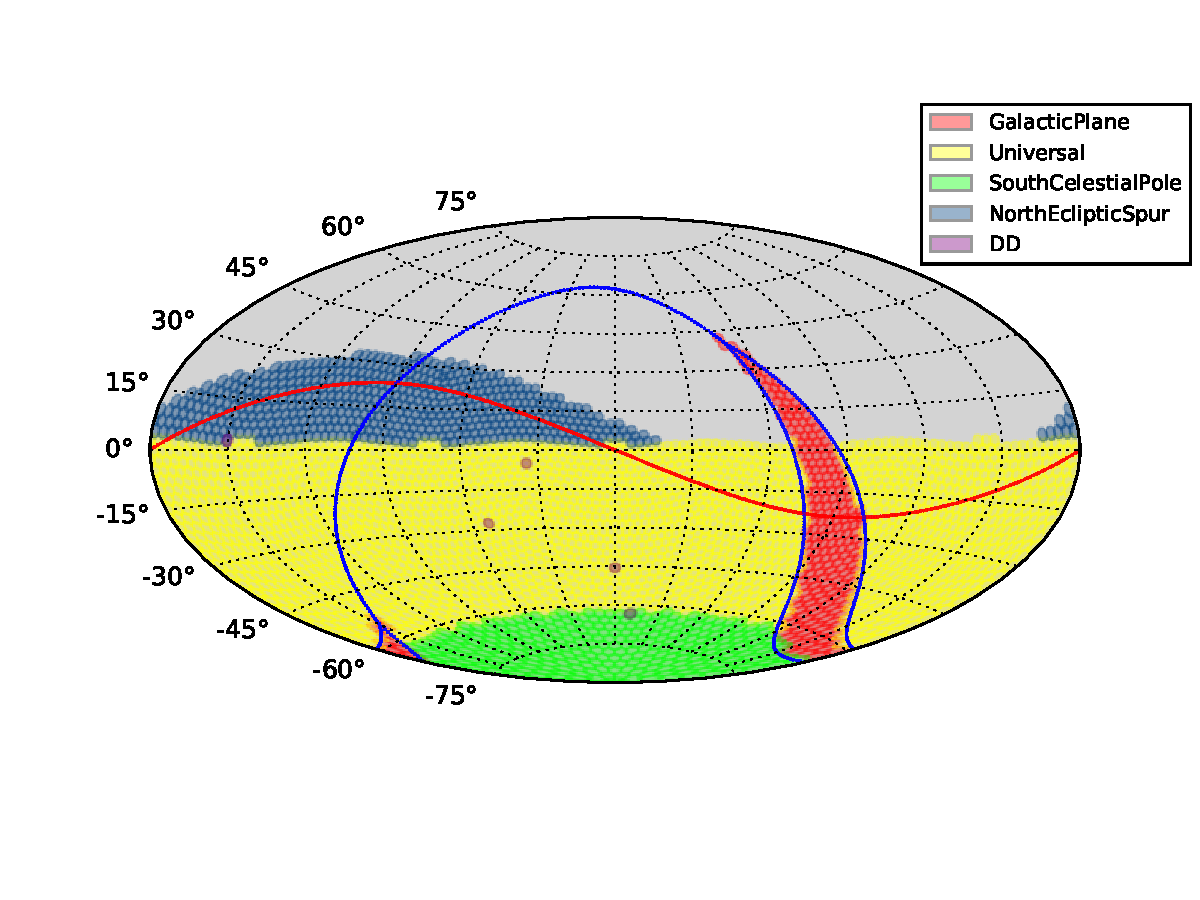
\includegraphics[width=.6\linewidth]{Figures/minion_1016_proposal_footprint.pdf}
%\plotone{Figures/minion_1016_proposal_footprint.pdf}
\caption{Regions of the sky with different requirements and constraints for scheduling: (1) Galactic Plane Region (GP), (2) Universal or Wide Fast Deep (WFD), (3) South Celestial Pole (SCP), (4) North Ecliptic Spur (NES), and (5) Deep Drilling Fields (DD). This figure is taken from \cite{jones2017large}.}
\end{center}
\end{figure}\label{fig_proposals}
The desirables and the constraints for different regions vary in both quantity and quality, see \cite{ivezic2008lsst} for a detailed explanation of the surveys associated with the sky regions. The notion of the features however, enables the scheduler to systematically fetch all of the various requirements and turn them into comparable quantities for the purpose of the decision making in the Markovian framework.\\
The proposed feature-space of the LSST contains seven features (see Section~\ref{sec_lsst_features} for the definition of features), each can be evaluated given a field $i$, a filter $f$, and a time $t$. The fields discretize the visible sky through a fixed partitioning with ID numbers preassigned to them. Each field can be captured through a single visit, that lasts for about 30 seconds. There are 6 possible filters, $[u,g,r,i,z,y]$, for a visit. And finally the time domain is discretized by the natural timing of the process. In other words, $t_j$ is exactly the moment that the $j$'th visit is over and the scheduler makes a decision for the next visit. Since a consecutive visit of the same field-filter is not allowed, there is a slew time between any two decisions, therefore $t_{j} - t_{j-1} > 0$. On the other hand, the operation is over a limited time horizon, $T$, thus the number of the decision time steps is finite. A finitely discretized sky, a finite number of the filters and a finite number of the time steps, define a finite feature-space, denoted by $\{(f_1(i,f,t_j)\dots f_7(i,f,t_j)): i = 1\dots n_f, f\in \{u,g,r,i,z,y\}, j = 0,\dots N\}$.
Then the implication of the policy, stated in Equation (\ref{equ_approx_pol}), for the LSST scheduler is as follows,
\begin{equation}\label{equ_approx_pol_imp}
\tilde{\pi}^*(x_j)= \argmin_{(i,f)\in \pazocal{A}_{j}} \sum_{k=1}^5 \theta^*_k E_{\pi}[\Phi_k(X_{j+1}) | x_j]\\,
\end{equation}
where $x_j = [f_{1, \dots,7}(id(t_j),ft(t_j),t_j)]$ is the 7-dimensional state at $t_j$, and $(i,f)$ is a feasible pair of field-filter. Section~\ref{sec_cstr} introduces the constraints under which a field-filter pair, $(i,f)$ is feasible at $t_{j}$. Accordingly, $\pazocal{A}_j$ is  the set of all field-filter pairs that are feasible at $t_j$.\\
Inline with the modular approach to the implementation of the scheduler, expected value of the basis functions, $E_{\pi}[\Phi_k(x_{j+1})|x_j]$ for $k=1,\dots, 5$ are evaluated in separated modules, developed by the LSST community. For instance, see \cite{sebag2008lsst} and \cite{sebag2007lsst}, for cloud cover measurements at the LSST site that were used to develop a cloud model and, see \cite{yoachim2016optical} for the sky brightness predictive model, specifically developed for the LSST. For the details of the basis functions of the Feature-Based scheduler for LSST refer to Section~\ref{sec_lsst_bfs}.\\
The last step is to implement the training procedures (described in Section~\ref{sec_opt}) on the LSST model to derive $\theta^*$. Training of the LSST scheduler is explained in Section~\ref{sec_lsst_opt} with adopting two sample objective functions. However, the LSST community, and basically any individual can design their own mission objective function, whether it allows for well-defined instant rewards or not, then train the scheduler through the open source training code, and find a new set of $\theta^*$ that principally leads to a different behavior of the scheduler due to different objectives.\\

\subsection{Features of the telescope scheduler}\label{sec_lsst_features}
For designing the features, it is important to avoid redundancy and ensure the inclusion of determining information. It is also critical to hold a modular approach in the delivery of the information to the decision procedure. For instance, consider the amount of time, $\Delta t$, it takes for a telescope to move on from a visit, characterized by a pair of $(i_1,f_1)$, to the next visit $(i_2,f_2)$,  where, $i_1$ and $f_1$ are the current field and the current filter respectively, and $i_2$ and $f_2$ are the next field and the next filter respectively. In LSST problem, $\Delta t$ mainly depends on the slew time, mechanical settling time, the dome placement time, and finally the time it takes to change the filter from $f_1$ to $f_2$. All of these timings are available through a precise simulation of the LSST model \cite{delgado2014lsst}. For all possible $(i_1,f_1)$, and $(i_2,f_2)$ a modular design would be to bring the summation of the operational timings to the stage of the decision, instead of bringing them separately as different features. This approach makes the implementation significantly simpler, more readable, and easier to debug, and in a conceptual level, makes it possible to track the effect of the operational timing in the overall outcome of the decision maker. Particularly, since the operational cost is independent of the amount to which each cause contributes to the overall $\Delta t$, bringing the timing of the separate procedures separately in the decision making level adds unnecessary complications to the design, and consequently, makes it hard to back track the output-input behavior of the scheduler. \\
This section proposes seven features for the description of the LSST-environment state in Table (\ref{tab_features}). They are designed to efficiently carry the determining information with a modular approach. Each feature is denoted by $f_k(i,f,t)$ for $k= 1..7$, and indexed by the triplet of $(i,f,t)$, field, filter, and time. To make a decision at $t$, the scheduler computes all of the seven features for all of the $(i,f)$ pairs in general, however, there are some features that don't change in every time step, for instance, if $i$ is not visited at $t^j$, then $f_5(i,f,t^j)= f_5(i,f,t^{j+1})$. For such cases, the implementation has a categorized updating procedure to avoid extra computations.
\begin{table}
\caption{Features of the approximated Markovian model for the telescope-environment system. Features $f_{1\dots 7}$ provide a memoryless, approximate description of the system's state.}
\begin{tabularx}{\textwidth}{|l|X|}
\hline
Notation & Definition\textbackslash Description\\ \hline \hline 
$f_1(i,f,t)$ & ($slew(id(t),i)+settling(id(t),i)+\Delta t_{f} I_{ft(t) \neq f} \vee t_{dome}(i)$): either the time required to point the telescope to $i$, and change the filter to $f$, or the time required to relocate the dome to make $i$ visible. Whichever that is larger.\\ \hline
$f_2(i,f,t)$ &  the total number of the same-night visits of field-filter $(i,f)$ until $t$.\\ \hline
$f_3(i,f,t)$ &  $(t - \tau_n(i,f,t)) I_{\{\theta(i,f,t) > \tau_s(t)\}}$, time since the last same-night visit of $(f,i),$\\ \hline
$f_4(i,f,t)$ &  remaining time for field-filter $(i,f)$ to become invisible, either by passing the airmass or the moon-separation threshold, or being covered by temporary objects such as clouds, as projected at $t$.\\ \hline
$f_5(i,f,t)$ &  co-added depth, a measure of cumulative quality of past visits of field-filter$(i,f)$ until $t$.\\ \hline
$f_6(i,f,t)$ &  $5\sigma$-depth, a measure for quality of visiting field-filter $(i,f)$ at $t$, depending on seeing, sky brightness, and airmass. $f_6(i,f,t) = C_m + 2.5 \log (\frac{0.7}{\sigma(i,t)}) + 0.50 (br(i,t)-21) - K(i,f) am(i,t)$ where $C_m$ is a scaling coefficient.\\ \hline
$f_7(i,t)$  & hour angle of field $i$ at $t$.\\ \hline
\hline
\end{tabularx}
\end{table}\label{tab_features}

\subsection{Basis functions of the telescope scheduler}\label{sec_lsst_bfs}
Basis functions are fully determined by the value of the features, and are denoted by $\Phi_k(f_1(i,f,t),\dots, f_7(i,f,t))$, for $k = 1 \dots 5$. Each $\Phi_k$, is indexed by a triplet of $(i,f,t)$, time, field, filter, and is evaluated at every decision making step, $t_j$, for all field-filter pairs $(i,f)$. Similar to the update procedure of the features, for a decision at time $t_j$, all six basis functions should be evaluated for all pairs of $(i,f)$, except for the field-filters that are infeasible at $t_j$. Feasibility of a field-filter can be evaluated after the evaluation of the features, by applying the constraints of the region that the field belongs to (see Section~\ref{sec_cstr} for the list of constraints). Thus, while it is required to evaluate the features for all possible pairs of $(i,f)$ at all decision steps, the number of the basis functions to be evaluated is on average approximately a factor of three less than the number of the features.\\
To incorporate the idea of features for the LSST scheduling problem with different requirements for different sky regions, we define a  set of common basis functions and then modify them according to the requirements of each region. 

\subsubsection{Common basis functions}
Generally speaking, making a decision for a visit at $t$ for the LSST scheduling problem is mainly determined by the following factors,
\begin{enumerate}
\item The amount of the time it takes to redirect the telescope and the dome to move from one target to the next target.
\item The short-term science-driven requirements, such as the same-night revisit of a field.
\item The long-term mission-driven requirements, such as maintaining a uniform coverage of all field-filter pairs within each region.
\item The relative quality of visiting a field-filter compared to other field-filters at the time of observation, for overall efficiency of the operation.
\item The general preference for observing the fields around the meridian.
\end{enumerate}
Accordingly, the basis functions of the LSST scheduler, are designed to formalize the above factors. Common basis functions that are shared amongst all of the regions, are defined in Table~\ref{tab_commonBF}.
\begin{table}[h]
\caption{Basis functions of the Feature-Based scheduler as the building blocks of the decision function.}
\begin{tabularx}{\textwidth}{| l | X |}
\hline
Notation & Definition\textbackslash Description\\ \hline \hline
$\Phi_1(f_1(i,f,t))$ & $s_1.f_1(i,f,t)$, the cost of the required time for visiting field-filter $(i,f)$.\\ \hline
$\Phi_2(f_2(i,f,t))$ &$\begin{cases}0.5,& \text{if } \sum\limits_{f}{f_2(i,f,t)} = 0\\ 1,& \text{if } \sum\limits_{f}{f_2(i,f,t)} = 2\\ 0,  & \text{else,}\end{cases}$, \newline reflects the short term visit/revisit priority of field $i$, conditioned on the total number of the previous same-night visits.\\ \hline
$\Phi_3(f_5(i,t))$ &  $(1 - \frac{f_5(i,f,t)}{\max_\iota \max_\phi f_4(\iota,\phi,t)})$, reflects the long-term visit priority of field-filter $(i,f)$, based on the ratio of its co-added depth to the maximum co-added depth of all pairs of field-filter until $t$.\\ \hline
$\Phi_4(f_6(i,f,t))$ & $1 - Pr(f_6(\iota,\phi,t) \leq f_6(i,f,t))$, empirical complimentary CDF of $5\sigma$-depth of all $(i,f)$ pairs at $t$. $\Phi_4$ assigns a cost to field-filter $(i,f)$ based on its relative visiting quality compared to the other field-filter pairs at $t$.\\ \hline
$\Phi_5(f_6(i,f,t))$ &  $\frac{|hr(i,t)|}{12}$, encourages visiting of the fields near the meridian.\\ \hline
\end{tabularx}
\end{table}\label{tab_commonBF}
In the definition of $\Phi_1$, scale factor $s_1= 0.43$ is empirically evaluated to ensure that 80\% of the observed values of this basis function for the winner states are between 0 and 1. Scaling the values of basis functions is a regulation that in general results in a faster rate of convergence in the training process of the scheduler, and does not harm the optimality of the solution.

\subsubsection{Region-specific modifications of the common basis functions}
As mentioned in Section~\ref{sec_lsst_problem}, the LSST's mission poses different requirements on different regions of the sky. This section presents how we modified the common basis functions to accommodate different desirables of the Wide Fast Deep (WFD), North Ecliptic Spur (NES),Galactic Plane Region (GPR), and South Celestial Pole (SCP)  surveys. Deep Drilling Field (DDF) survey, however, contains a very small fraction of the visible sky's area, thus for the relatively rare event of the DDF observation, instead of modifying the policy we prescribe a schedule, and interrupt the operation of the scheduler. Particularly because, the recoverability attribute of the Feature-Based scheduler enables the scheme of the interruptions to be a part of the decision making procedure. In other words, if the interruptions are not too frequent, the Feature-based scheduler will recover itself back to the normal behavior, without requiring any information about the decisions before the interruption. \\
\begin{table}[h!]\label{tab_regionBF}
\caption{Adjustments of the basis functions based on the requirements of each region.}
\begin{tabularx}{\textwidth}{| X | X |}
\hline
Modified basis functions & Description\\ \hline \hline
$\Phi_2^{\text{WFD}}(f_2,f_3,f_4) =$ \newline $\begin{cases} \Phi^{\text{pair}}(f_3)I_{f_4> W_2},& \text{if } \sum\limits_{f}{f_2} = 1,\\ \Phi_2(f_2),& \text{else } \end{cases}$ \newline\newline $\Phi_2^{\text{NES}}(f_2,f_3,f_4) =\Phi_2^{\text{WFD}}(f_2,f_3,f_4)$ \newline\newline $\Phi_2^{\text{GPR}}(f_2) = \Phi_2(f2)$ \newline\newline $\Phi_2^{\text{SCP}}(f_2) = \Phi_2(f2)$\newline\newline $\Phi^{\text{pair}}(f_3) :=$ \newline $\begin{cases} \exp(- \frac{\min_{\phi}f_3(i,\phi,t)}{W_2})& \text{if } \min_{\phi}f_3(i,\phi,t) < \frac{W_2}{2}\\ 0, & \text{else}\end{cases}$ 
& The WFD and NES surveys require pairs of visits for which a second same-night visit has to be scheduled in a certain time window, $[W_1,W_2]$. $ \Phi^{\text{pair}}$ is defined to encourage second valid visits. There is no revisit strategy for GPR and SCP fields because they receive at most one visit per night in the baseline LSST mission, hence no modification is required.\\ \hline
$\begin{array}{l c l}\Phi_3^{\text{WFD}}(f_5) &=& s_{WFD} \Phi_3(f_5)\\ \Phi_3^{\text{NES}}(f_5) &=& s_{NES} \Phi_3(f_5)\\ \Phi_3^{\text{GPR}}(f_5) &=& s_{GPR} \Phi_3(f_5)\\\Phi_3^{\text{SCP}}(f_5) &=& s_{SCP} \Phi_3(f_5)\end{array}$ 
& The total number of the required visits is different for fields in different surveys, to take this difference into account, we set $s_{WFD} = 1$, and scale the third basis function of other regions according to the ratio of the required visits with respect to the required visits of the WFD survey.\\ \hline
\end{tabularx}
\end{table}

%
%\subsubsection{Controllability of the scheduler}\label{sec_sim_cont}
%
%As discussed in Section~\ref{sec_SM}, the mission's objective has to be controllable via the design parameters, $\theta$. In this section we present an empirical observation of the mission's objective controllability. If the value of the objective function does not sufficiently respond to the variations of the design parameters, it is a sign of poor choice of the basis functions and/or input information. Either of these factors lead to a structure that does not admit a sufficiently optimal solution, and if on the other hand, the objective function is extremely variable with respect to the changes in the design parameters, the solution of the training is not reliable because the objective is not a well-behaved function of the optimization variables.
%
%Fig~\ref{fig_controlability}, shows a few one dimensional slices of the two following simple objective functions (\ref{equ_short_term_U1}) and (\ref{equ_short_term_U2}), evaluated after about five hours of scheduling simulation, with different $\theta$'s in $[0,10]$ range. To observe the variability of the objective function with changes in the $i$'th basis function, we define a sequence of equidistant values for $\theta_i \in \{\theta_i^{j_1},\dots,\theta_i^{j_m}\}$ and keep the other $\theta$'s fixed, then run the scheduler for $T = 4.8 hrs$ with all resulting $\theta$'s that are different by the $i$'th element, then evaluate $U_1$, and $U_2$, defined as follows. $U_1$ reflects the slew time $slew(.)$ and airmass $am(.)$ aversion, and $U_2$ reflects the time-efficiency of the operation.
%
%\begin{equation}\label{equ_short_term_U1}
%U_1(x_0,x_{1}, \dots, x_{n})= -\sum_{\{i:t_0<t^i<t_n\}} {slew(id(t_{i}), id(t_i)) + 10 . am(id(t_i))}
%\end{equation}
%
%\begin{equation}\label{equ_short_term_U2}
%U_2(x_0,x_{1}, \dots, x_{n})= n
%\end{equation}
%
%
%
%
%\begin{figure}[h]
%\begin{center}$
%\begin{array}{ll}
%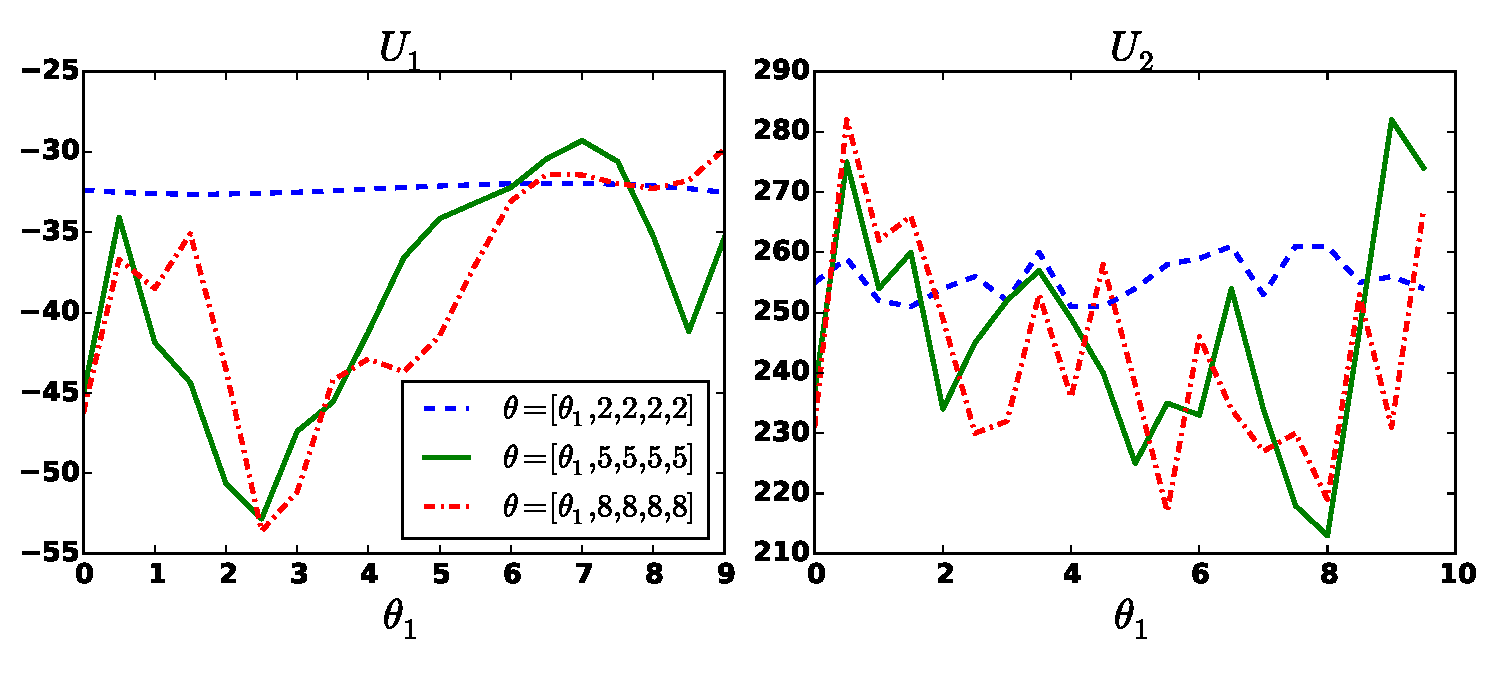
\includegraphics[width=.5\linewidth]{Figures/Theta1.pdf}&
%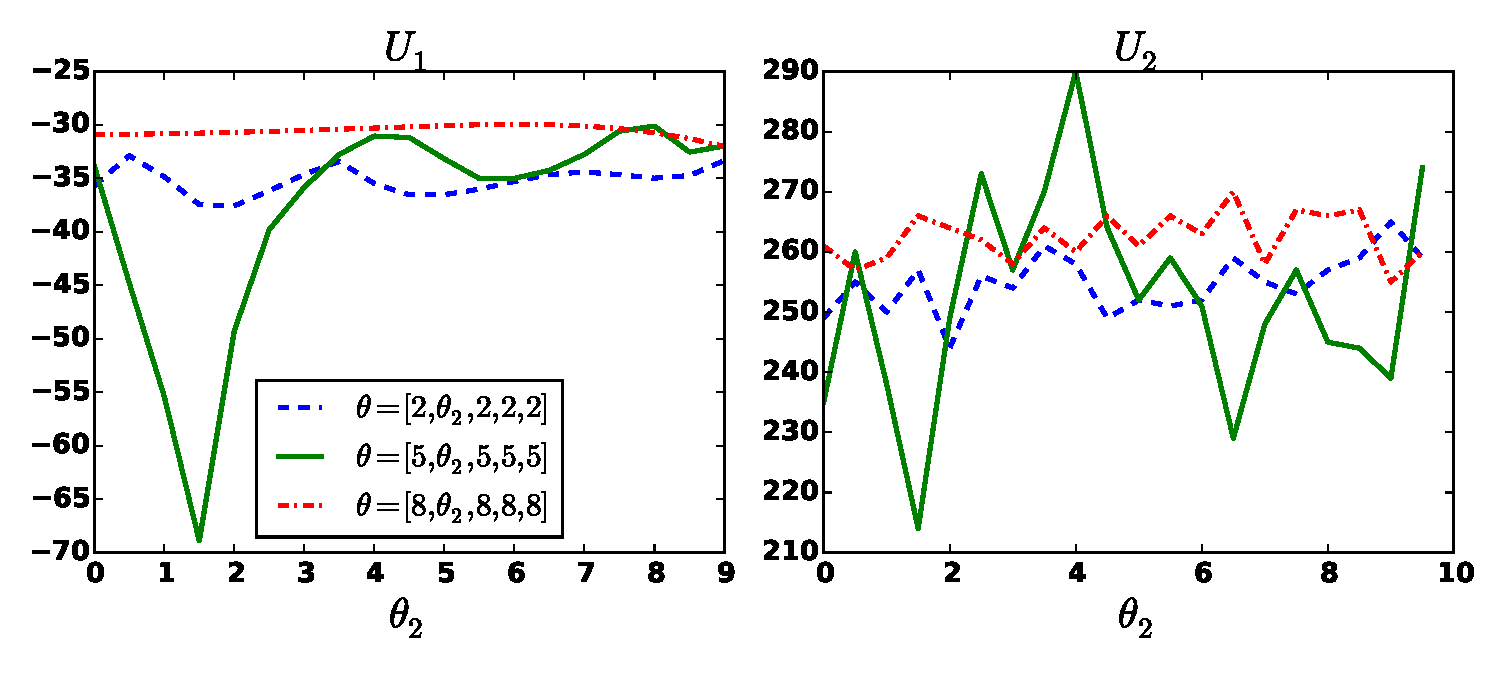
\includegraphics[width=.5\linewidth]{Figures/Theta2.pdf}
%\end{array}$
%\end{center}
%
%\begin{center}$
%\begin{array}{ll}
%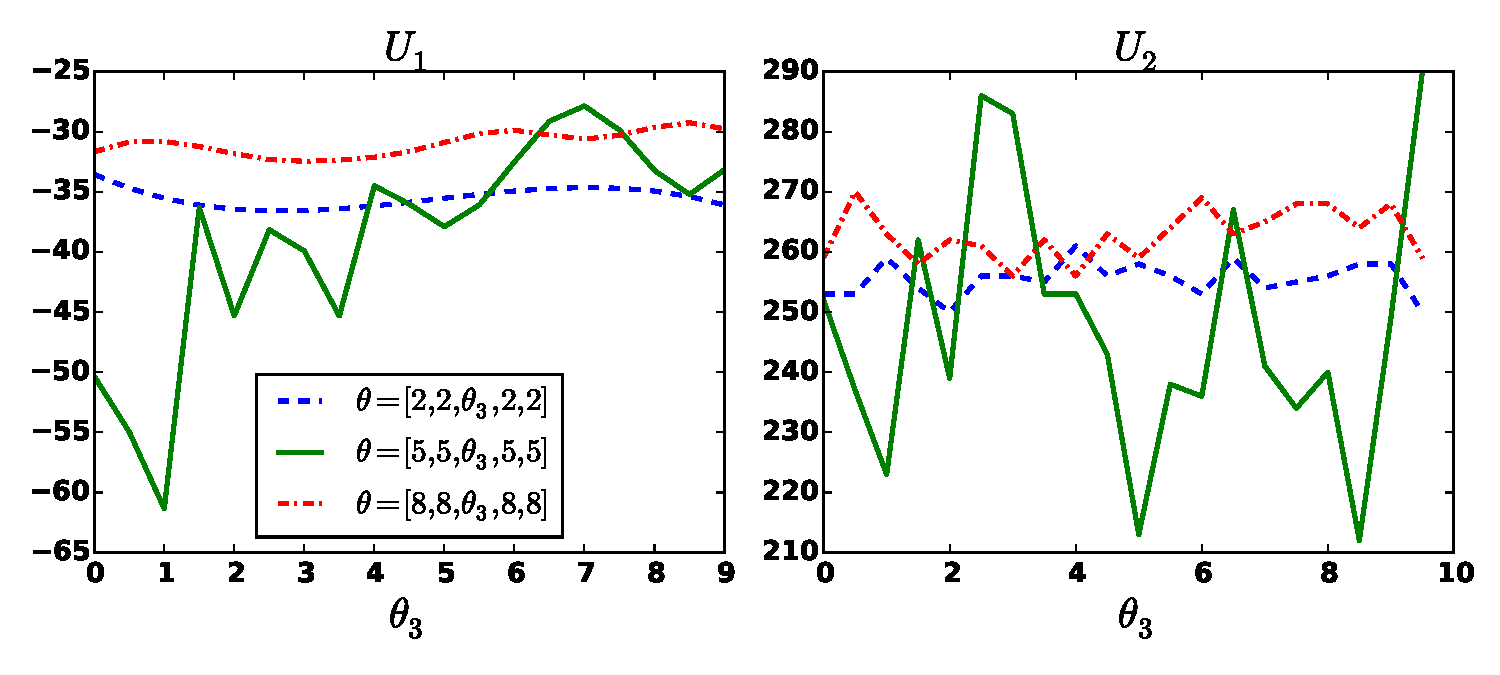
\includegraphics[width=.5\linewidth]{Figures/Theta3.pdf}&
%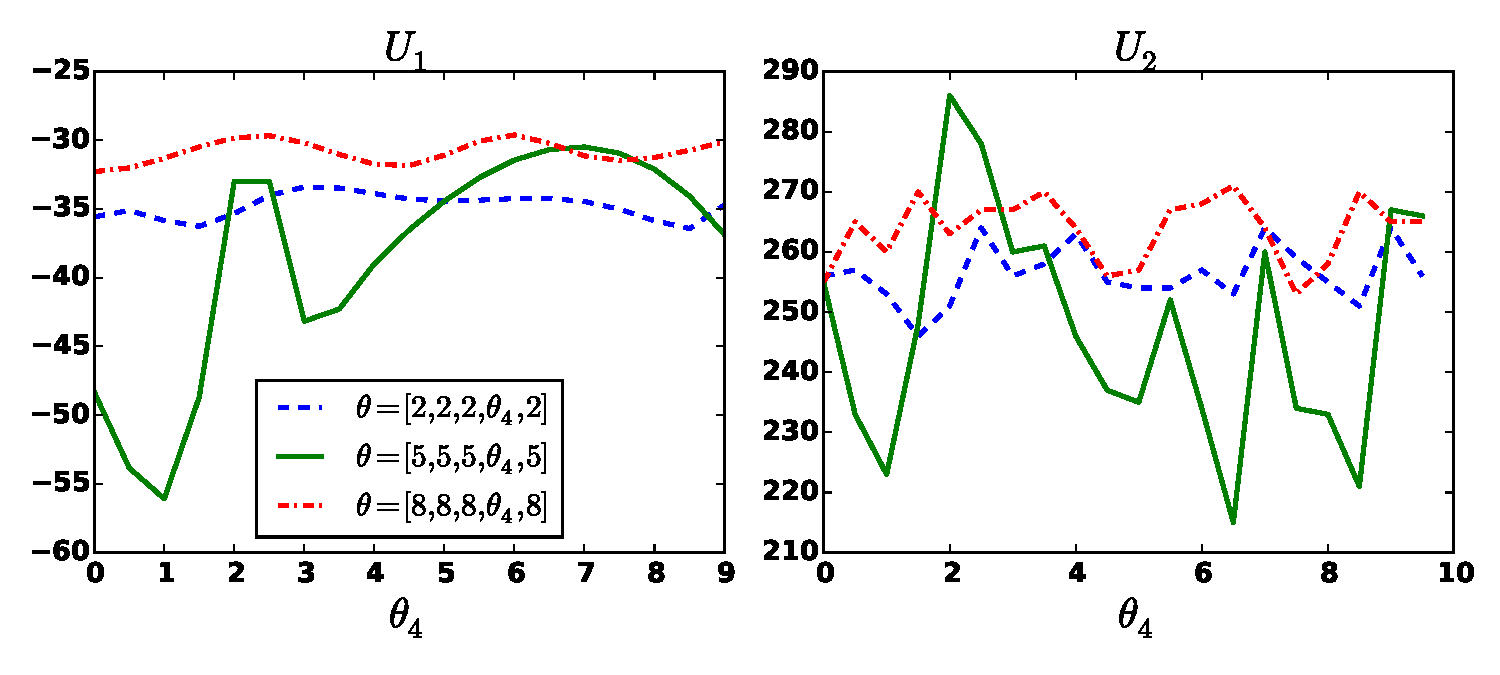
\includegraphics[width=.5\linewidth]{Figures/Theta4.pdf}
%\end{array}$
%\end{center}
%
%\begin{center}$
%\begin{array}{l}
%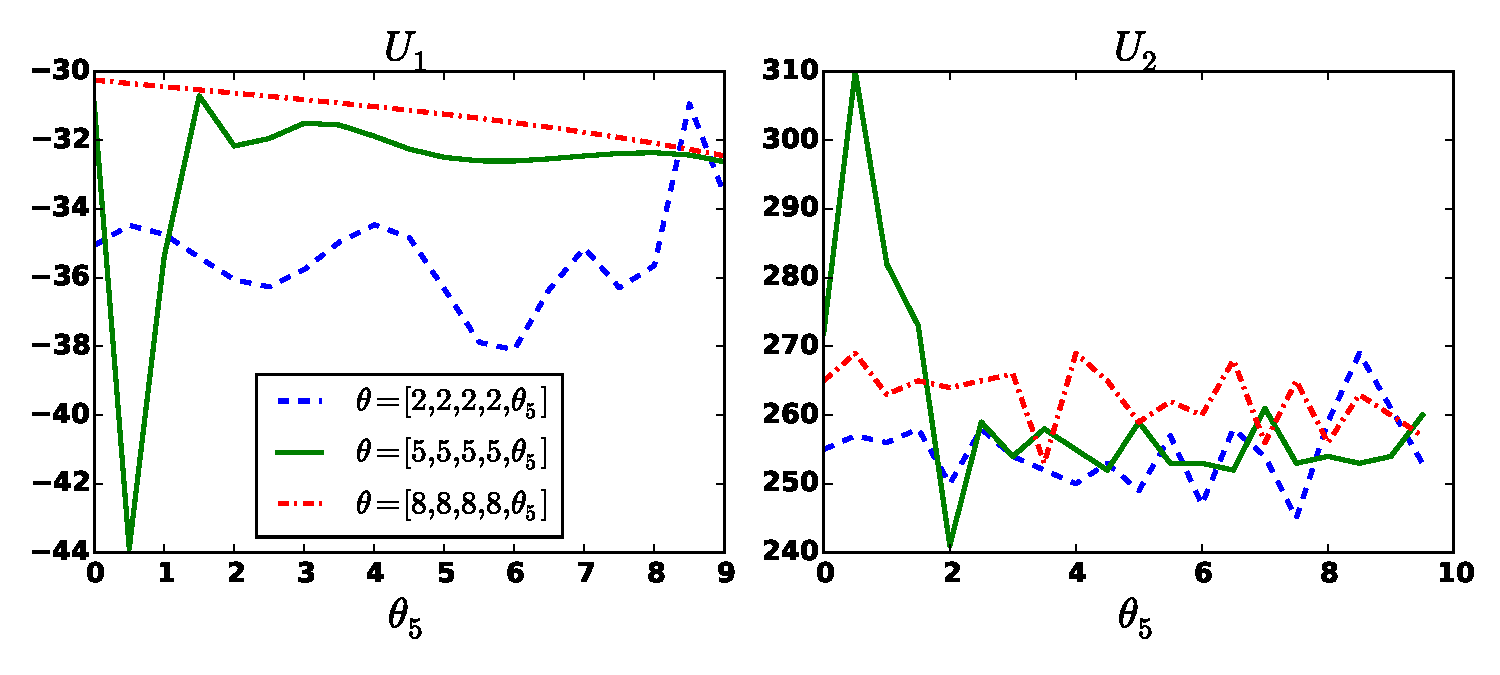
\includegraphics[width=.5\linewidth]{Figures/Theta5.pdf}
%\end{array}$
%\end{center}
%
%\caption{One dimensional slices of the two simple objective functions (\ref{equ_short_term_U1}) and (\ref{equ_short_term_U2}). The variation of the objective functions, specially in the mid-range slices (solid line) suggests that the scheduler's performance is controllable with the design parameters $(\theta_1,\theta_2,\theta_3,\theta_4,\theta_5)$ within the proposed range of the search. This is of course valid for the performance that is measured with either of $U_1$, or $U2$.}
%\label{fig_controlability}
%\end{figure}
%
%
%
%
%Figure~\ref{fig_controlability}, contains slices of the 5-dimensional $U_1$ and $U_2$. Both of the simple objective functions and the total number of visits reasonably respond to the changes in all five dimensions of the variable $\theta$, which can be an evidence of the controllability of the objective function. Moreover, the smaller variations for slices closer to the boundaries of the search space, suggest that the design and scaling of the basis functions provide a desirable behavior for the objective function within the proposed search space.
%

\subsection{Survey-specific constraints}\label{sec_cstr}
The scheduler's decision at each time step is an admissible (feasible and measurable) pair of field-filter $(i,f)$, thus before each decision, one needs to specify the set of feasible actions. Feasibility of a candidate pair is driven by the following measurable factors:
\begin{itemize}
\item Visibility: The candidate field-filter has to be visible.
\item Quality: The expected observational quality of a field-filter has to be beyond the given lower threshold.
\item Survey's timing: The science-Driven revisit constraints has to be respected.
\end{itemize}
Exact expression of the proposed constraints for the LSST scheduler are presented in Table~\ref{tab_feasibility}.
\begin{table}[h!]
\caption{Feasibility of field-filter $(i,f)$ for a visit at $t^{n+1}$, as evaluated at $t^n$.}
\begin{tabularx}{\textwidth}{| l | X | X |}
\hline
& Constraints& Description \\ \hline \hline
1&$ \tau_{rise}(i,f,t^{n+1}) \leq t^{n+1} \leq \tau_{set}(i,f,t^{n+1}) $ & field-filter $(i,f)$ has to be above the acceptable airmass horizon at $t^{n+1}.$ \\ \hline
2&$ E[f_4(i,f,t^{n+1})] \neq 0 $ & field-filter $(i,f)$ is not temporarily masked at $t^{n+1}$. \\ \hline
3 & $\sum_{f}f_2(i,f,t^n) < N^{\textit{survey}}$ & $N^{\textit{survey}}$ poses a region dependent upper-bound on the number of the visits for each field. $N^{WFD}= N^{NES} = 3$, and $N^{GPR}= N^{SCP} = 1.$ \\ \hline
4 & $E[f_6(i,f,t^{n+1})] < \sigma({\textit{survey},f})$ & the expected quality of visiting field-filter $(i,f)$ at $t^{n+1}$ has to be better than the given threshold, $\sigma(.)$, that depends on the survey and the filter. \\ \hline
5&$f \neq id(t^n)$ & consecutive visit of a same field is not allowed. \\ \hline
6& if $\sum_{f}f_2(i,f,t^n) = 0$ then \newline $\max_\phi f_4(i,\phi,t^n) > \frac{W_1+W_2}{2}$ & the first visit of field $f$ has to occur $\frac{W_1+W_2}{2}$ time before it becomes invisible, so that the second visit of $f$ can be scheduled in the valid time window.  (WFD and NES only)\\ \hline
7& if $\max_{\phi}\theta(i,\phi,t^n) > \tau_s(t^n)$ then \newline $ W_1 \leq \min_{\phi}f_2(i,\phi,t^n) \leq W_2 $& if there has been a same-night visit of field $f$ until $t^n$, then the next same-night visit has to occur in the valid time window. \\ \hline
8&if \newline $\max_{\phi}\theta(i,\phi,t^n) > \tau_s(t^n)$ then \newline $f \notin \{\text{y},\text{u}\}$ & if there is a same-night visit of field $f$ until $t^n$, then the next same-night visit cannot be with either of u or y filters. (WFD only)\\ \hline
9& $f \notin \{\text{y},\text{u}\}$ & visits with u filter and y filter is not allowed. (NES only)\\ \hline
\end{tabularx}
\end{table}\label{tab_feasibility}

\section{Scheduler optimization}\label{sec_lsst_opt}
For both of the reinforcement learning and the global optimization approaches, discussed in Section~\ref{sec_opt} we used a simulated model of the telescope and the environment, including the brightness model of the sky and coverage of the clouds, developed based on the measurements at the LSST site. 

\subsection{Reinforcement training}
The simulation for the reinforcement learning starts at $t_0 = 2462867.5~mjd$ (January 1, 2021), with $\theta^0 = (5,5,5,5,5)$, initialized at the mid-range values, and continues until $\theta$ converges. Figure~\ref{fig_theta_conv}, is the training curve for all of the variables over a course of 3000 decisions, for the following instant reward. The discount rate of $\gamma = 0.9$, and learning rate of $\frac{0.01}{\log^3(i)}$ are chosen empirically. 
\begin{equation}
r(s_{i-1}, s_i) = -slew(id(t_{i-1}), id(t_{i})) - am(id(t_i))
\end{equation}
\begin{figure}[h!]
\begin{center}
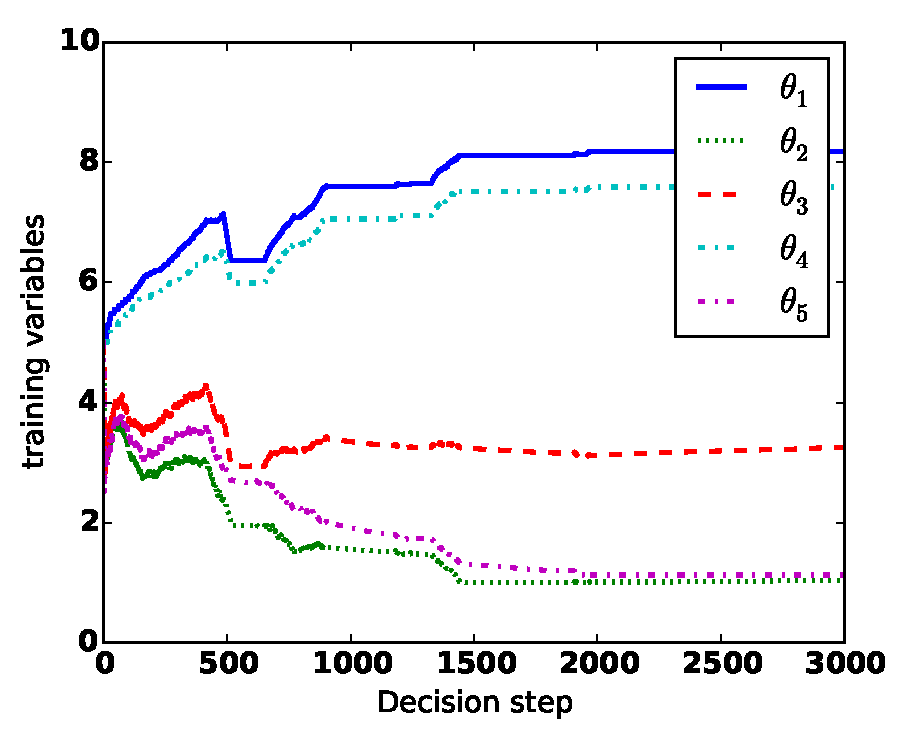
\includegraphics[width=0.5\linewidth]{Figures/TDcurve.pdf}
\end{center}
\caption{Reinforcement learning of the scheduler's parameters, $(\theta_1,\theta_2,\theta_3,\theta_4,\theta_5)$. All of the parameters are initialized at the mid-range value, 5. During the simulation, at each step there is a cost associated with the decision which implies a small adjustment on each of the five parameters. Then the next decision will be taken with a slightly different set of variables. This procedure continues until the adjustments on the variables are negligible.}
\label{fig_theta_conv}
\end{figure}
For the above choices of reward, learning rate, discount factor and initialization, $\theta$ converges to $\theta^* = (8.18,  1.04,  3.26,  7.59,  1.13)$.
In this approach, the computational time to evaluate the update is negligible with respect to the time required to evaluate the features, therefore, the computational time of the reinforcement learning is almost equal to the scheduling simulation (without the updates on $\theta$) which is linear with respect to the number of the decisions. With a personal computer \footnote{Processor: 1.6 GHz, Memory: 4 GB 1600 MHz DDR3}, each decision takes about $0.5$ second, thus the time of the convergence for the simulation, presented in this session is $3000\times 0.8 \text{ sec } = 40 \text{ minutes }$.

\subsection{Global optimization}\label{sec_globalopt}
One of the important simple objective functions that cannot be expressed as the discounted sum of the rewards is the total number of the observations from any $t_i$ to any $t_j$,
\begin{equation}\label{equ_lsst_ede}
U_{\pi_{\theta}}(x_i, x_{i+1}, \dots, x_j) = j - i.
\end{equation}
To find a set of parameters $\theta$ that optimize the above objective function we applied the global optimization approach, explained in \ref{sec_gopt}, with the following regulatory constraints:
\begin{itemize}
\item $\theta \geq 0$: The basis functions, $\Phi_i(.), i = 1\dots 5$, are designed to reflect the operational cost, therefore a linear combination with positive coefficients $\Phi(s_{t^n})= \sum_{i=1}^5 \theta_i \Phi_i$, would reflect the overall cost of the operation that we minimize in our policy.
\item $\theta_1 =\theta_0$: We fix the value of the the first element of $\theta$ to reduce the dimension of the optimization problem by one. This is possible without the loss of generality because each element of $\theta$ does not have a meaningful inherent value, and in fact, its value compared to the other elements determines the behavior of the policy. In other words, if $\theta^*$ yields an optimal scheduler, then $\alpha \theta^*$ for $\alpha > 0$ yields an optimal scheduler due to the homogenous of the policy (\ref{equ_approx_pol}), where, 
\begin{equation*}
\argmin_{a_{i}} \sum_{j=1}^k \theta^*_j E[\Phi_j(X_{i+1}) | a_{i}] = \argmin_{a_{i}} \sum_{j=1}^k \alpha \theta^*_j E[\Phi_j(X_{i+1}) | a_{i}].
\end{equation*}
\end{itemize}
We used the objective function (\ref{equ_lsst_ede}) for $t_i = 2462867.5~mjd$ (January 1, 2021) and $t_j = 2462877.5~mjd$ (January 11, 2021). Figure~\ref{fig_eDEObjectiveFunction}, shows the value of the objective function over the iterations of the $e$DE algorithm. The solution $\theta^* = (1.00, 0.84, 0.99,  1.34,  3.04)$, yields the best $U_{\pi_{\theta}}$ after 50 iterations for $\theta_1 = 1.00$

\begin{figure}[h!]
\begin{center}
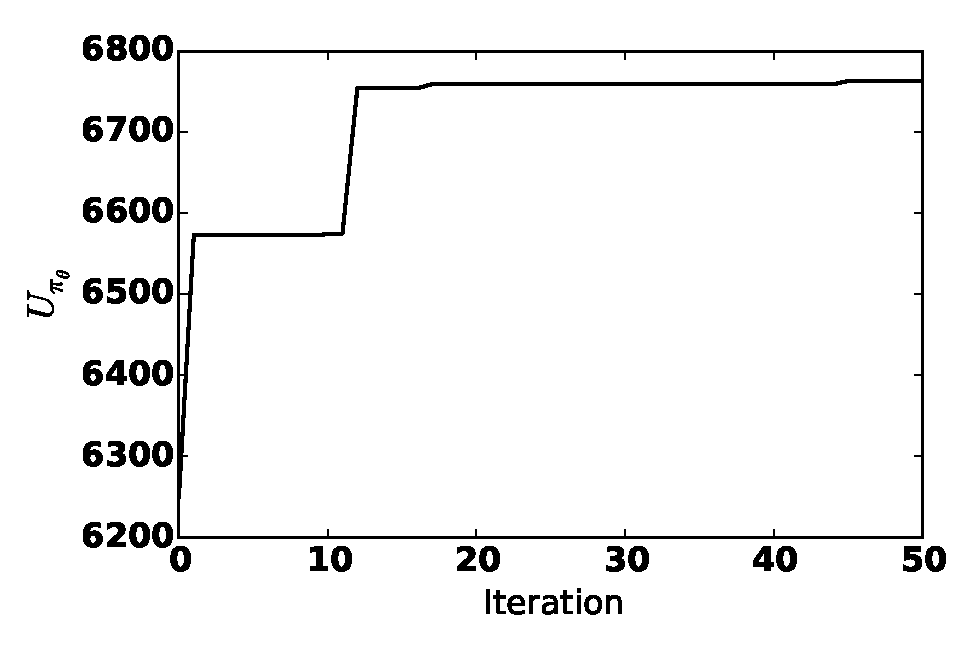
\includegraphics[width=0.4\linewidth]{Figures/eDEObjectiveFunction.pdf}
\caption{Progress of the objective function over the iterations of the $e$DE algorithm. $U_{\pi_{\theta}}$, for this simulation is the total number of the observations in 10 nights of simulated scheduling.}
\label{fig_eDEObjectiveFunction}
\end{center}
\end{figure}
$e$DE is a population-based metaheuristic algorithm, and for the result shown in Figure~\ref{fig_eDEObjectiveFunction}, number of the population $N_P$ is set to be 50. Each function evaluation is in fact, the simulation of 10 days of scheduling with a candidate scheduler which takes about 8 minutes, therefore each iteration, in total, takes $N_P * 8$ minutes with a personal computer\footnote{Processor: 1.6 GHz, Memory: 4 GB 1600 MHz DDR3}. The optimization can be manually terminated if the result is satisfactory, or can be continued until a full convergence. In $e$DE (and all genetic algorithms in general), function evaluation for each individual is independent from other individuals, therefore the parallel implementation of the same algorithm can be faster up to a factor of $N_p$. 

\section{Performance of a modified Feature-Based scheduler for LSST}\label{sec_comp}
In this section, the LSST Metric Analysis Framework \cite{jones2014lsst} is used, to compare \footnote{The sky background models and weather downtime used to benchmark the algorithms are not exactly identical because of the practical difficulties in the separation of the environment and the scheduler in the \textit{astro-lsst-01-2013}'s implementation. However, for the purpose of the comparisons in this paper, the behavior of our sky and observatory model is sufficiently close to the official model.} the performance of a modified version of the Feature-Based scheduler with \textit{astro-lsst-01-2013}, the most recent official schedule of the LSST, over a 10-year period of scheduling simulations.\\
The Modified Feature-Based scheduler is under active development\footnote{GitHub repository: \url{https://github.com/lsst/sims_featureScheduler}.}, and addresses the observational details of the LSST's mission through the adjustment of the constraints and the basis functions. It is designed to produce a software that can be used in practice. In this version, we adopt a finer discretization of the sky using high resolution HEALpixel maps and do not require the partitions to be necessarily sized based on the telescope's field of view. The fact that the policy is not computationally expensive to evaluate makes it possible to use finer discretization of the state space. This approach allows the scheduler to handle the field's overlaps that cause inhomogeneity in the coverage of the sky. In addition to adopt a finer discretization, we use a spatial dithering scheme to randomize the final pointing of the telescope by a small amount around the center of the partitions, to further assist the homogeneity of the coverage. Moreover, the Modified Feature-Based scheduler uses a separate process tracking if an observation will need to be observed in a pair, and a separate processes deciding if a deep drilling sequence should be executed.\\
%For the Modified Feature-Based scheduler, we use five basis functions:
%
%\begin{enumerate}
%\item{A map showing how much time it would take to slew to given positions in the sky.}
%\item{A penalty for changing filters. This penalty is lifted when twilight starts or stops and when the moon rises or sets.}
%\item{A HEALpix map that tracks how many observations have been taken across the sky and compares it to an ideal coverage map.}
%\item{A map of the current 5$\sigma$ limiting depth minus the 5$\sigma$ depth map of when a point is on the meridian in dark time. This effectively combines throughput considerations based on the current sky brightness, airmass, and filter choice.}
%\item{A mask which limits where the telescope can slew in altitude and azimuth, including mechanical exclusion areas and exclusion areas around the moon and bright planets.}
%\end{enumerate}
For a survey telescope, such as LSST, the density of the co-added depth over the visible sky has to be ideally uniform in each filter and within each of the five survey regions. Figure~\ref{fig_10yrs_skymap} compares the values of the co-added depth on a (finely) discretized sky map after a 10-year period of scheduling simulation. Figure \ref{fig_zoomin_g}, compares the smoothness of the co-added depth coverage in a smaller scale for each scheduler in the \textit{g} band as an example, however the granular coverage pattern of \textit{astro-lsst-01-2013}, and smooth coverage of the Modified Feature-Based scheduler is similar for all of the filters. Smoother coverage that the Modified Feature-Based scheduler offers is due to the fine discretization of the sky, hence the state-space of the Markovian model, and the dithering scheme. \\
Figure~\ref{fig_10yrs_hist} and compares the distribution of the co-added depth on a (finely) discretized sky. The Modified feature-Based scheduler has paved the left-most peak that appears in the distribution of \textit{astro-lsst-01-2013}. This peak is the result of the field's overlaps that receive more number of visits than it's assumed in the decision making procedure of the scheduling. The default sky tessellation adopted by LSST results in 23\% of the sky being covered by more than one field. Adopting the dithering scheme, the median number of observations at a typical point in the sky increases by $\sim15$\%. Dithering is also essential for removing systematic effects for science cases such as measuring galaxy counts \cite{Awan2016}.
\begin{figure}[h!]
\begin{center}$
\begin{array}{ll}
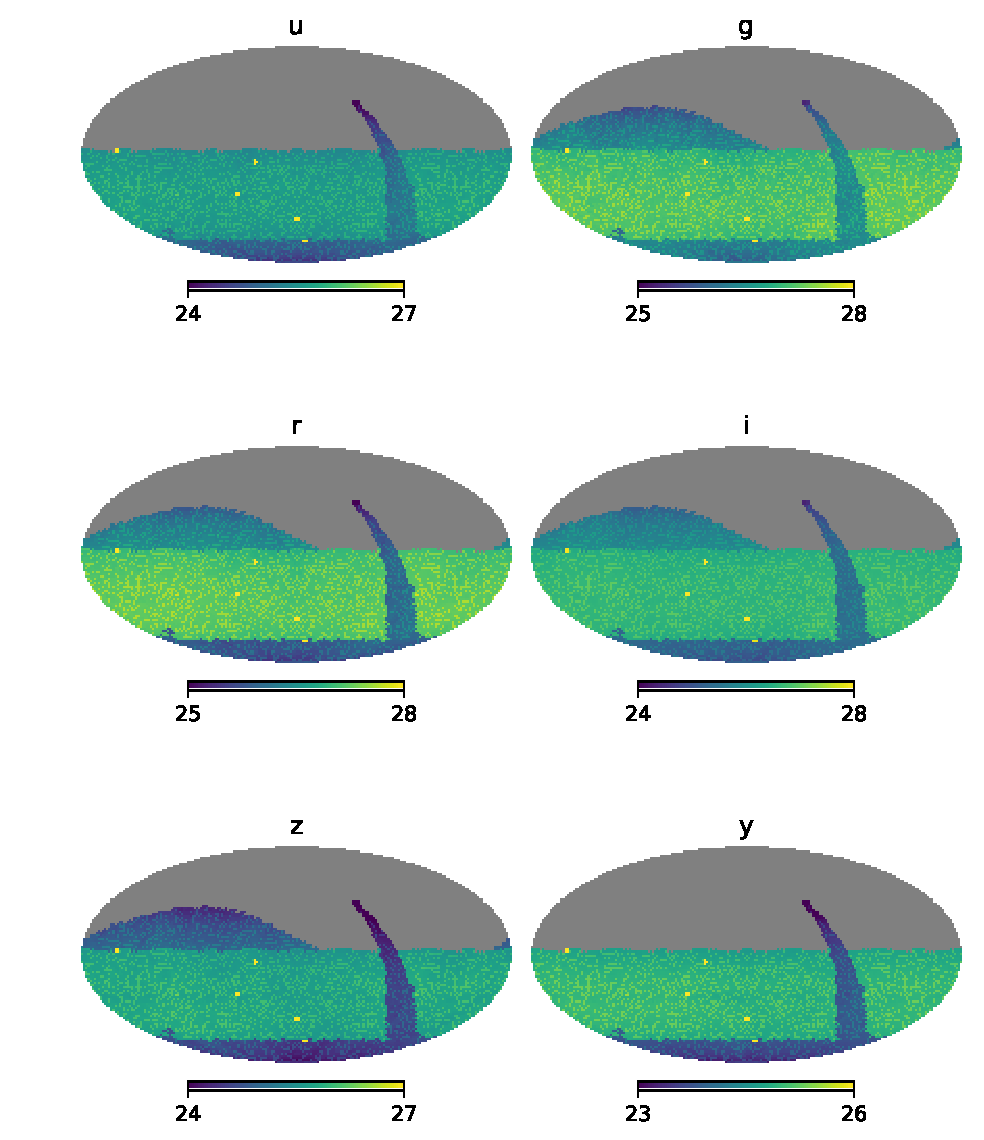
\includegraphics[width = 0.45\textwidth]{Figures/OpSim10yrs_skymap.pdf}&
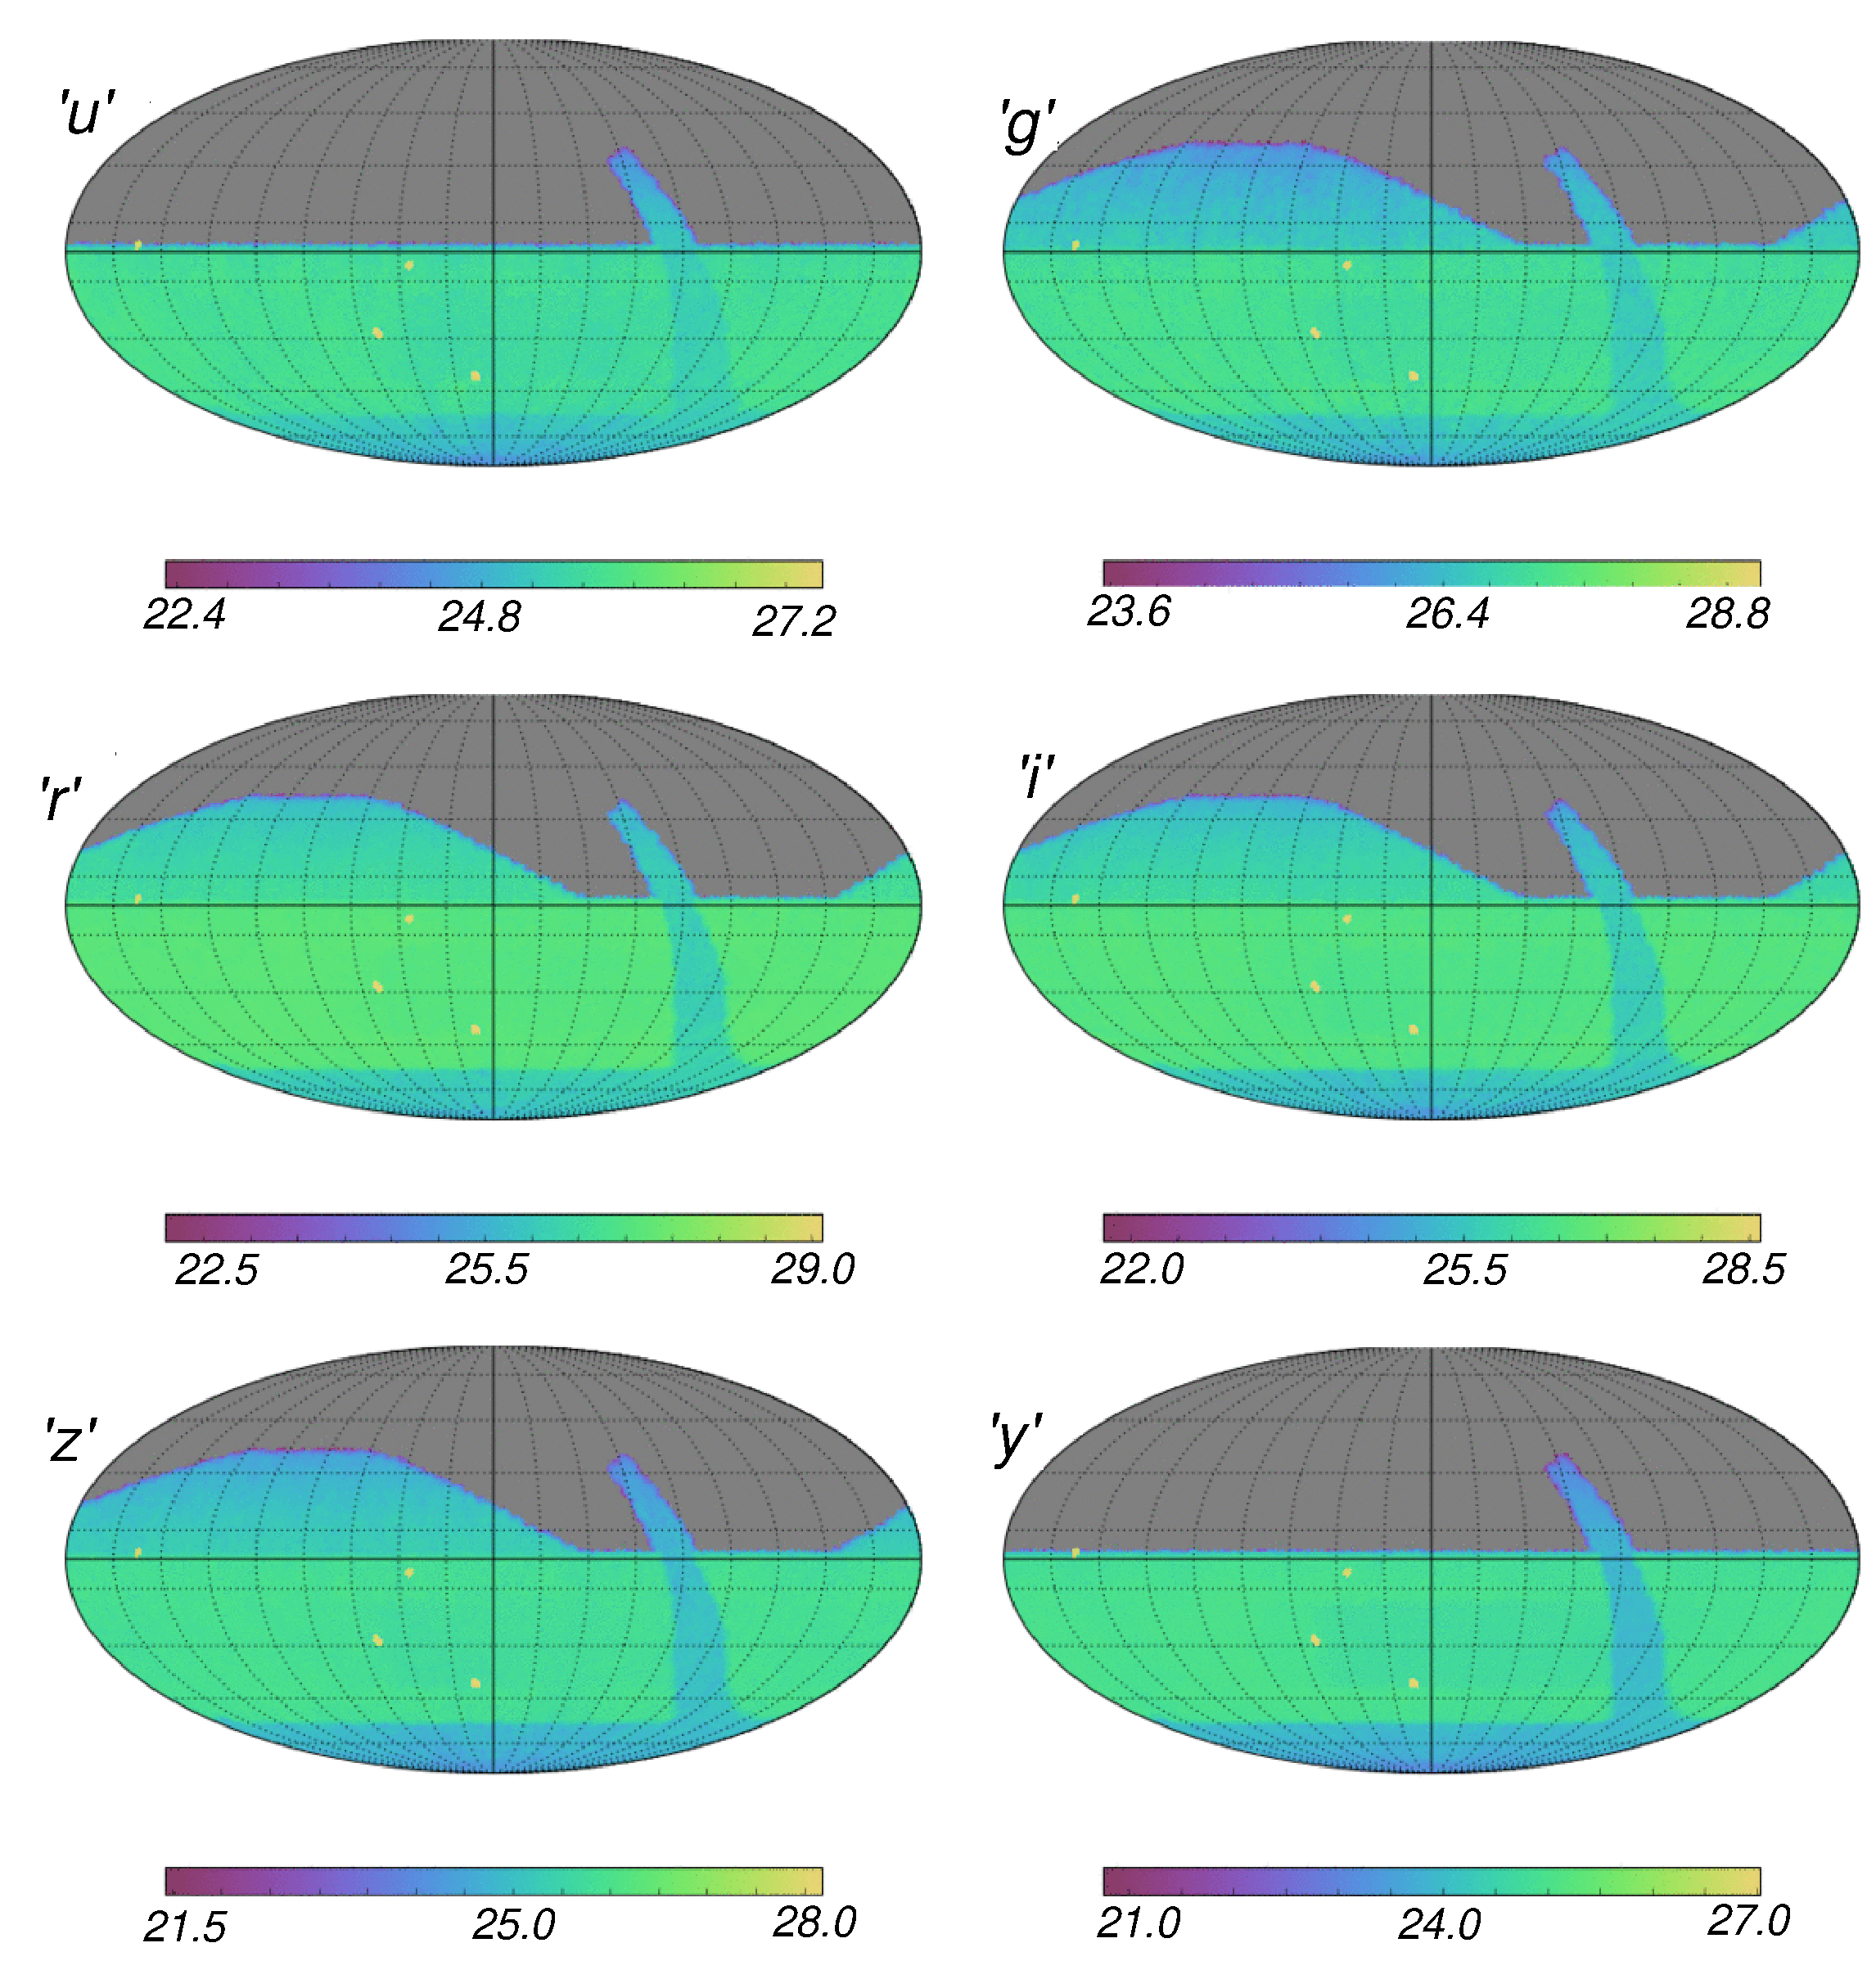
\includegraphics[width = 0.45\textwidth]{Figures/FB10yrs_skymap.pdf}\\
\end{array}$
\end{center}
\caption{The final co-added depth coverage in each of the six filters $\{ u, g, r, i, z, y\}$. According to the mission's objective, the scheduler has to provide a uniform coverage of the visible sky within each region, and in each filter. The left panels show the \textit{astro-lsst-01-2013} simulation results while the Modified Feature-Based scheduler is on the right. Modified Feature-Based scheduler closely matches the footprint of the official survey, and because of its adjustability property, offers a systematic way to de-emphasize the regions, that in the mission definition, are decided to be de-emphasized, such as the galactic plane and south celestial pole.}
\label{fig_10yrs_skymap}
\end{figure}
\begin{figure}[h!]
\centering
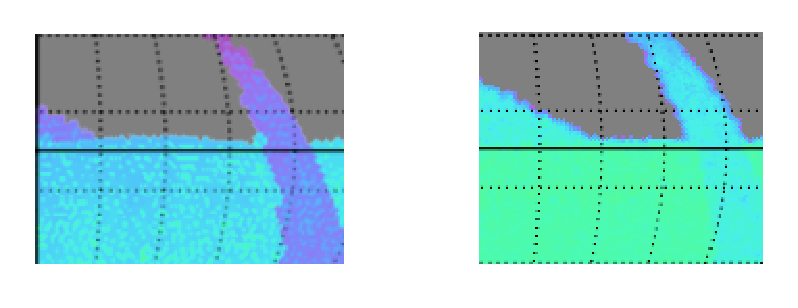
\includegraphics[width=0.5\linewidth]{Figures/ZoominG}
\caption{Smoothness of the co-added depth coverage in a smaller-scale, in the \textit{g}-band. The smooth coverage of the Modified Feature-Based scheduler (right) versus the granular pattern of \textit{astro-lsst-01-2013} (right), furthur satisfies the uniformity of the coverage which is one of the most fundamental objectives of the LSST mission.}
\label{fig_zoomin_g}
\end{figure}
\begin{figure}[h!]
\centering
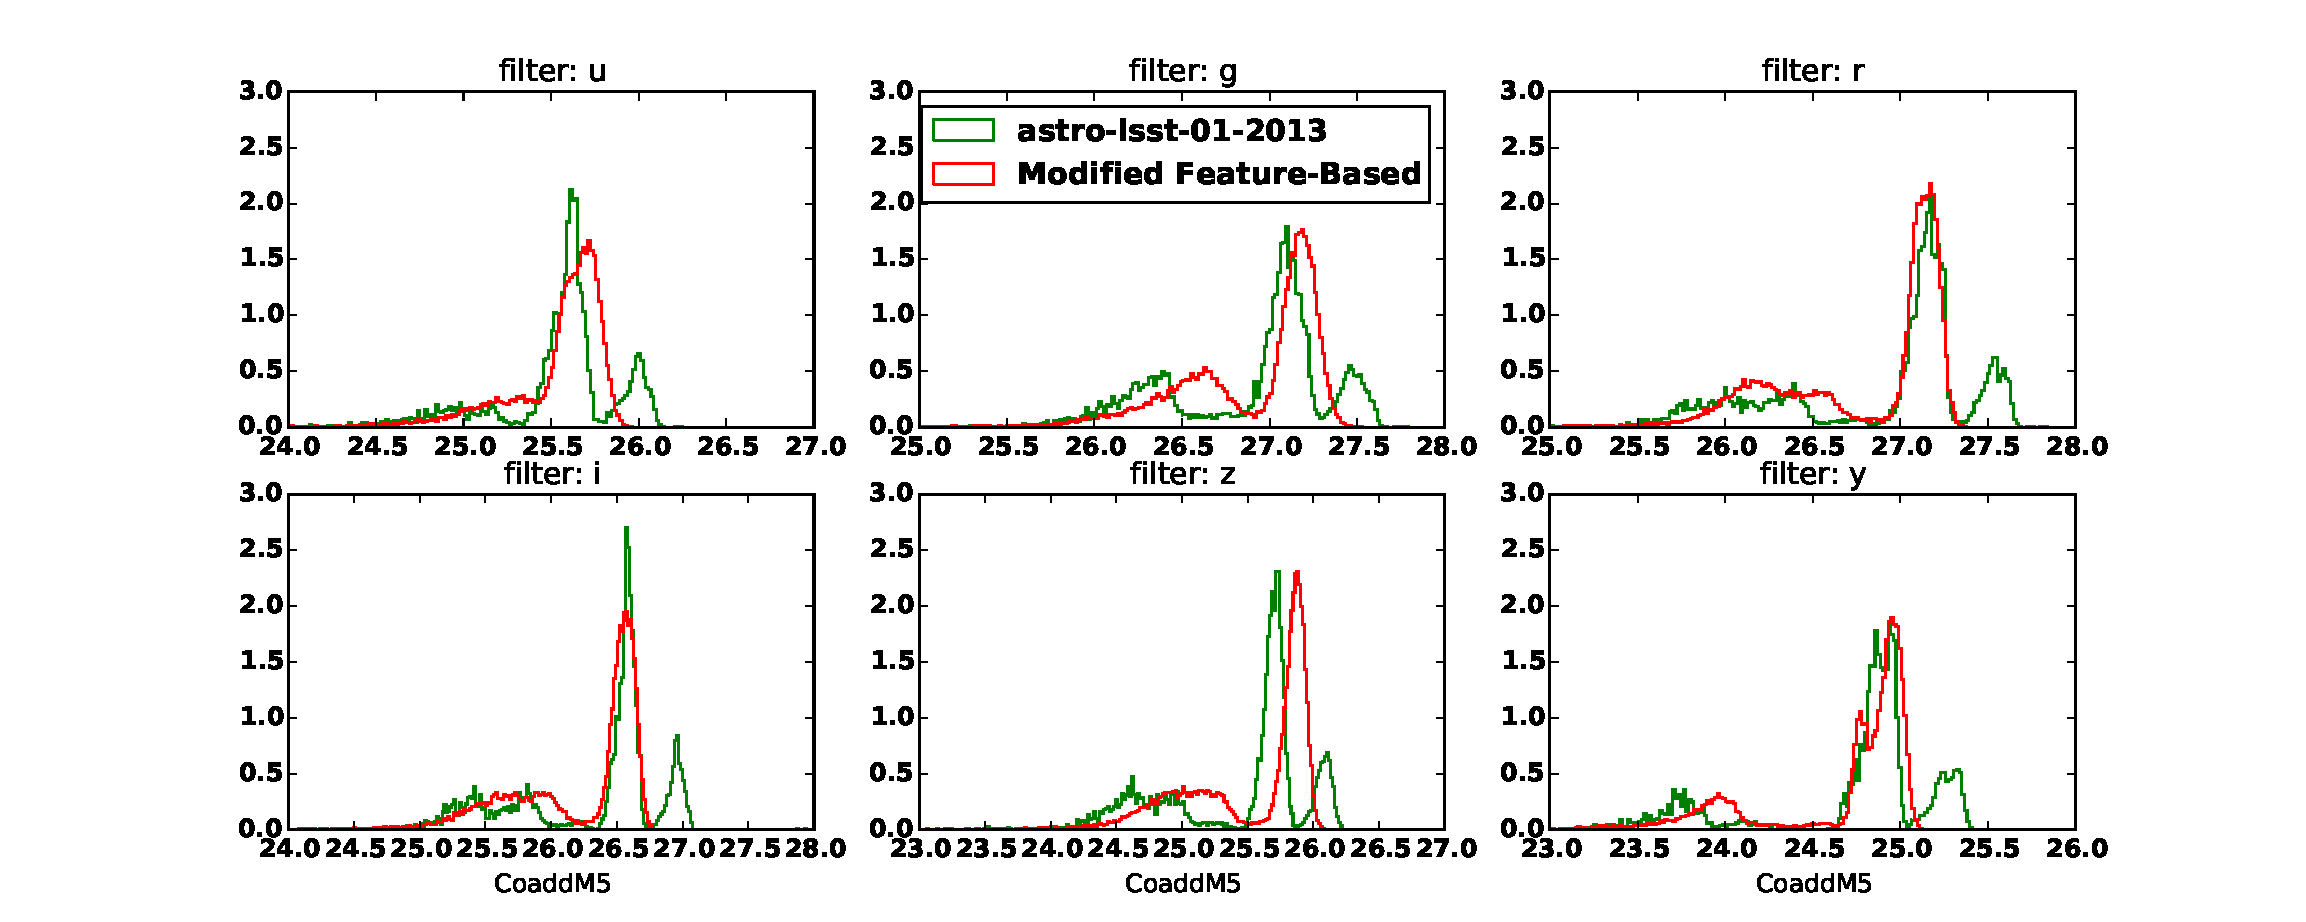
\includegraphics[width=1.0\linewidth]{Figures/Co_addedHist10yrs.pdf}
\caption{Each plot compares the distributions of the co-added depth coverage in one of the six filters. A dithering scheme in the Modified Feature-Based scheduler smoothens the depth of the coverage where the fields overlap. Consequently and in contrast with \textit{astro-lsst-01-2013}, one cannot find an extra unwanted peak on the right extreme of the distribution. As a consequence of paving the overlap peak, the telescope's time is spent on improving the median of the depth coverage distribution that amounts to a higher co-added depth for a larger area of the sky.}
\label{fig_10yrs_hist}
\end{figure}
%\begin{table}\label{table_10yrs_hist}
%\caption{The median and variance of the co-added depth distribution on a finely discretized sky. Modified Feature-Based scheduler closely matches the footprint of the official survey, and in addition outperforms \textit{astro-lsst-01-2013} in terms of the uniformity of the coverage, with lower variances, specially in WFD and SCP regions.}
%\begin{center}
%\resizebox{\textwidth}{!}{%
%\begin{tabular}{l|cccc|cccc} \hline
%&\multicolumn{8}{c}{Median, Variance} \\ \hline
%&\multicolumn{4}{c|}{\textit{astro-lsst-01-2013}} &\multicolumn{4}{c}{Modified Feature-Based} \\
%filter  & WFD & GP & SCP & NES & WFD & GP & SCP & NES\\
%\hline
%\textit{u}& 25.63, 0.04 & 25.12, 0.11& 24.91, 0.12& - &25.68, 0.01 &25.32, 0.05 & 25.10, 0.04& -\\
%\textit{g}& 27.13, 0.04 & 26.41, 0.09& 26.32, 0.12 & 26.30,0.13& 27.18, 0.01 & 26.69, 0.04&26.56, 0.04 &26.47, 0.09 \\
%\textit{r}& 27.19,0.04 & 26.01,0.16& 25.84,0.24 & 26.38, 0.12 & 27.14, 0.01& 26.21, 0.07 & 26.08, 0.05 & 26.43, 0.09\\
%\textit{i}& 26.60, 0.04 & 25.44, 0.15 & 25.28, 0.22 & 25.82, 0.12 & 26.56, 0.01 & 25.68, 0.08 & 25.43, 0.07 & 25.88, 0.09\\
%\textit{z}& 25.73, 0.04& 24.62,0.17& 24.57, 0.21& 24.90, 0.14 & 25.87, 0.01 & 25.03, 0.9 & 24.81, 0.05 & 25.16, 0.10\\
%\textit{y}& 24.92, 0.04 & 23.81, 0.16 & 23.72, 0.21& - & 24.92, 0.02 & 24.01, 0.09 &23.88, 0.06 & -\\
%%all & 157.2, 1.37&151.4, 11.94& 150.6, 6.32&103.4, 11.1&157.4, 0.38 & 153.0, 2.12&151.9, 1.56& 104.0, 1.40\\
%\end{tabular}}
%\end{center}
%\end{table}
%%%%%LSST's mission calls for uniform coverage of the sky and prefers a smaller variance in the distribution of the final co-added depth. 
In addition to uniformity of the coverage, the LSST mission calls for pairs of visits within a valid time window at the same night. The main reason is to detect the transient objects such as asteroids. Since, the moving objects usually belong to the solar system, the pair constraint was initially imposed only on the WFD and NES regions. However, there are interesting solar system objects such as interstellar asteroids that can be observed in any direction of the sky, besides identification of the other varying objects, such as super novae, can benefit from a follow up visit, especially if the second visit is with a different filter. Thus in the Modified Feature-Based scheduler we made the pair constraint a universal constraint for all of the regions.The downside of this extension is the fact that it constrains the scheduler even more and the performance can be potentially less than it could be. Note that the structure of the Feature-Based scheduler, allows for extension or restriction of the constraints down to the individual field's level, with neither contradicting any of the Markovian framework assumptions, nor breaking the structure of the implementation. Figure~\ref{fig_10yrs_pair_hist} demonstrates the distribution of the observations in pair (in the $g$, $r$, and $i$ filters) to the total number of the observations. For the regions that the pair constraint is applied, this ratio can be interpreted as the success rate of the scheduler to satisfy the pair constraint. Note that the peak of the density for Figure~\ref{fig_10yrs_pair_hist} is closer to $1$, which means a larger area of the sky is covered by successful visits-in-pairs, however, the Modified Feature-Based scheduler offers a sharper concentration of the values that can be interpreted as a more homogenous visits-in-pair ratio. In other words, the Modified Feature-Based scheduler, sacrifices perfect visit-in-pair for a limited area of the sky to maintain a uniform ratio of visit-in-pair for a larger area of the sky.\\
%\begin{figure}[h!]
%\begin{center}$
%\begin{array}{ll}
%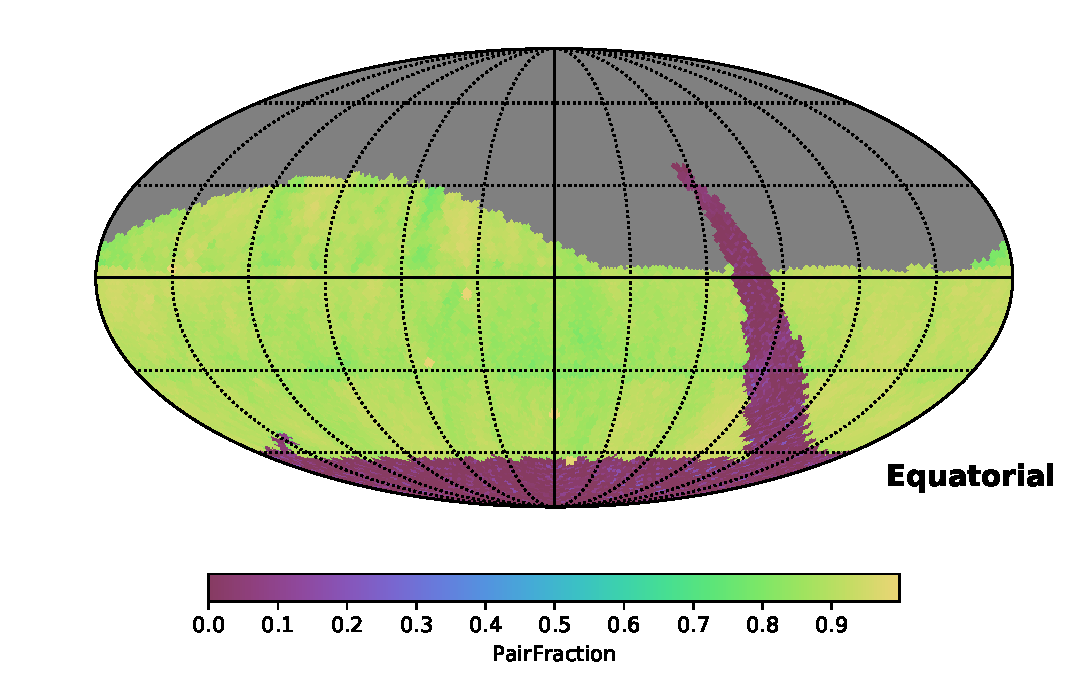
\includegraphics[width = 0.45\textwidth]{Figures/OpSim10yrs_Pair_skymap.pdf}&
%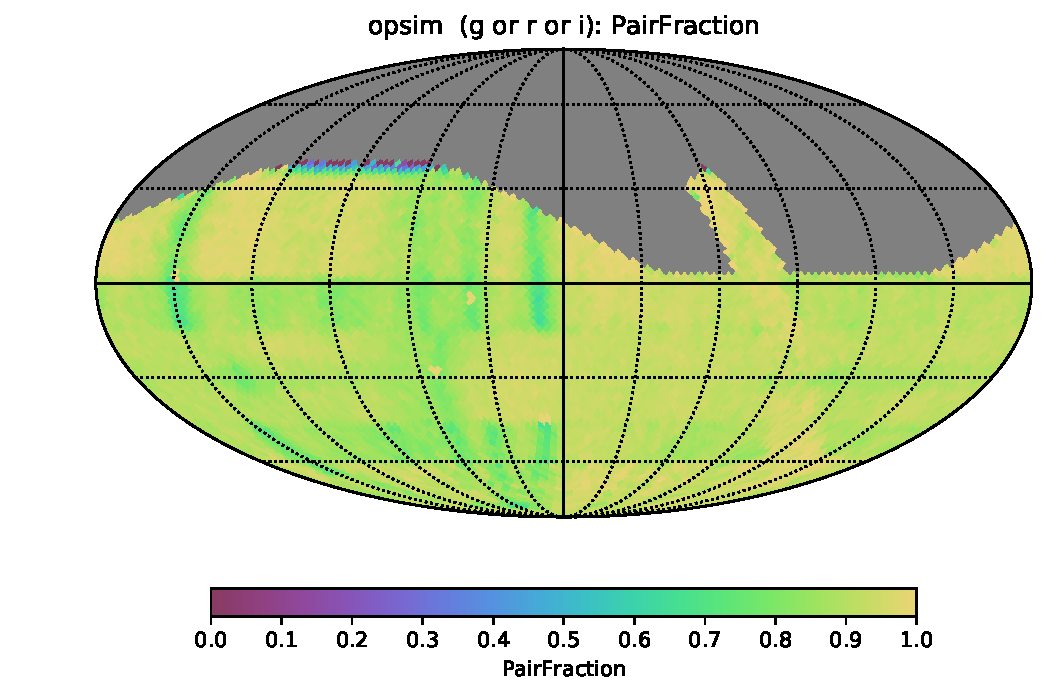
\includegraphics[width = 0.45\textwidth]{Figures/FB10yrs_Pair_skymap.pdf}\\
%\end{array}$
%\end{center}
%\caption{The ratio of the visit-in-pairs (in the $g$, $r$, and $i$ filters) to the total number of the observations on the sky map. For the areas that the pair constraint is applied, the ratio is desired to be one. For Modified Feature-Based scheduler (right), the pair constraint is applied to all of the regions and for \textit{astro-lsst-01-2013} (left), it is applied to the WFD and NES regions only.}
%\label{fig_10yrs_pair}
%\end{figure}
%
\begin{figure}[h!]
\centering
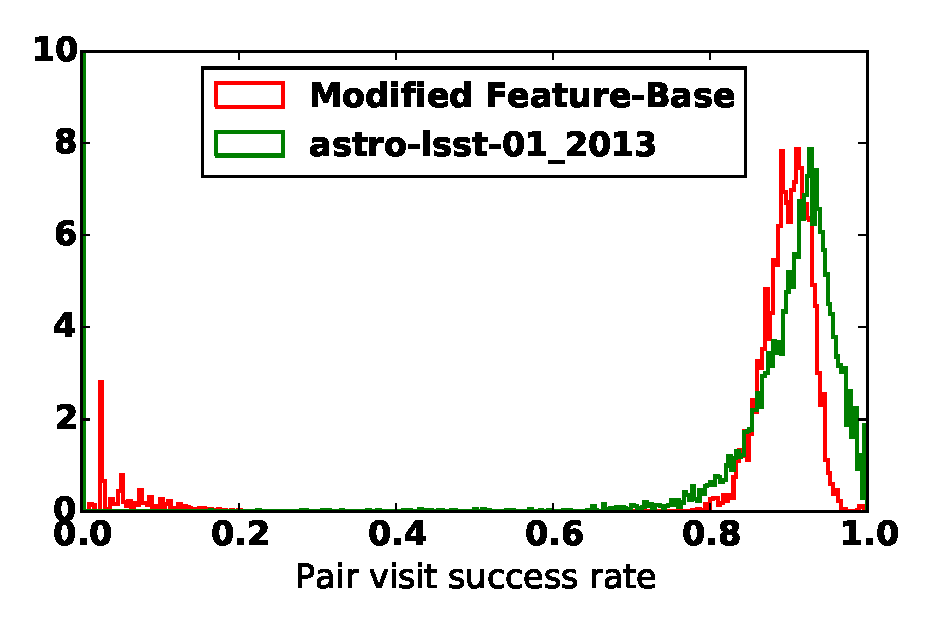
\includegraphics[width=.4\linewidth]{Figures/PairHist.pdf}
\caption{Distribution of the visits-in-pair ratio to the total number of the observations, in any of the \textit{g}, \textit{r}, and \textit{i} filters. The Feature-Based scheduler in compare with \textit{astro-lsst-01-2013}, sacrifices perfect visit-in-pair for a limited area of the visible sky (with a lower mean) to maintain a uniform ratio of visit-in-pair for a larger area of the sky (with a sharper distribution)}
\label{fig_10yrs_pair_hist}
\end{figure}
%For a ground-based instrument, airmass is one of the major obstacles for high-quality observation. Although zenith observations have the minimum airmass, off-zenith observations cannot be avoided, in which case, observations around the meridian provide high quality data and consequently more efficient operation of the telescope. Figure~\ref{fig_10yrs_AltAz} compares the number density of the visits on an altitude-azimuth sky map in each of the six filters $[u,g,r,i,z,y]$. Clearly in all of the filters, the modified Feature-Based scheduler schedules more visits around the desirable meridian zone. In addition, it offers a consistent concentration peak on the east wings, which is essential for a higher success rate for the visit-in-pair constraint. Because, if the first visit of the night occurs when the field is on the east side of the sky, it provides a longer time opportunity for the second visit of the same night. Note that adjustability of the Feature-Based scheduler allows for a significant change in the behavior, in this case a variant of the marching army cadence is incorporated to control the location of the visits through a basis function modification.
For a multi-mission, survey telescope, such as LSST, comparing the performance of the different schedules is a difficult task. Particularly because of the large number of the competing factors that are involved in the performance evaluation. In some cases involving the importance of each area of astronomy, the criteria are not even objective. We conclude this section with a general comparison by combining the surveys' open shutter fraction (OSF), and median airmass of the observations. The open shutter fraction is the total time that the telescope camera shutter was open divided by the total time it could have been open. This reveals how time-efficiently the observations have been scheduled. The median airmass reflects the overall quality of the collected data. Generally speaking, observations in lower airmass allows for a higher data quality. Figure~\ref{fig_all_alt_az} visualizes the number density of the visits on an altitude-azimuth sky map for the modified Feature-Based scheduler with the most recent LSST baseline schedules \textit{astro-lsst-01-2013} and \textit{minion\_1016}. Table~\ref{OSF_table}, shows that there is a trade-off between airmass and OSF. For instance \textit{minion\_1016}, offers the best OSF (time efficiency), while the median armass is the worst (data quality). Meanwhile \textit{astro-lsst-01\_2013} offers low airmass abservations, resulting in a lower OSF. Moreover, in the $r$\ filter where atmospheric extinction is less relevant, \textit{minion\_1016} has a higher total throughput while \textit{astro-lsst-01\_2013} has higher throughput in the $g$\ filter. By including dithering, the modified Feature-Based scheduler vastly outperforms the other surveys in both the blue and red filters. The Modified Feature-Based simulation has the lowest OSF, but this is an initial simulation where the basis function weights have not been optimized, so there is potential for further improvements. Moreover using the Modified Feature-Based scheduler for observations in large blocks could improve the OSF as shown in D. Rothchild et al. (2018, in preparation).\\
\begin{table}\label{OSF_table}
\caption{Comparison of three different survey algorithms in a section of the WFD region.}
\begin{center}
\begin{tabular}{lccccc}\hline
Survey& OSF & median Airmass & dithered & \multicolumn{2}{c}{median throughput}\\
  & &&& $r$ (\%) & $g$ (\%)\\ \hline \hline
Modified F-B & 0.705 & 1.1 & yes & 63.7 & 47.0 \\
minion\_1016 & 0.736 & 1.2 & no & 55.3 & 40.0 \\
astro-lsst-01\_2013 & 0.715 & 1.1 & no & 54.4 & 40.8 \\ \hline
\end{tabular}
\end{center}
\end{table}
%
%
%\begin{figure}[h!]
%
%\begin{center}$
%\begin{array}{rl cc rl}
%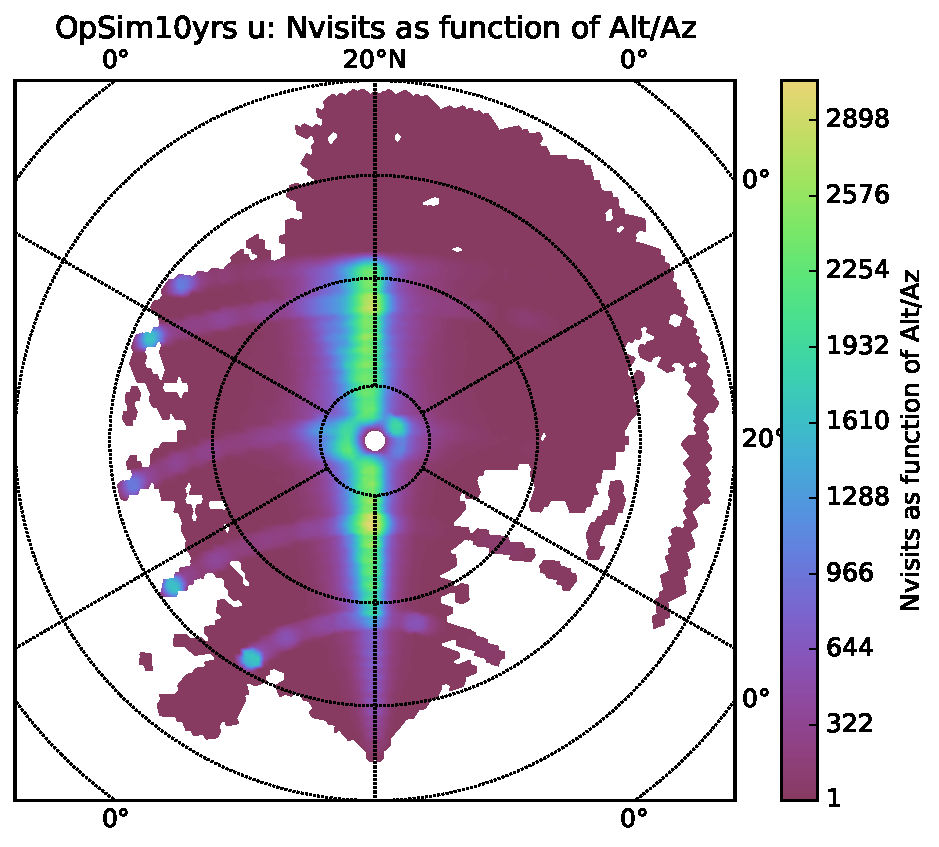
\includegraphics[width=.25\linewidth]{Figures/opsim_Nvisits_as_function_of_Alt_Az_u_HEAL_SkyMap.pdf}&
%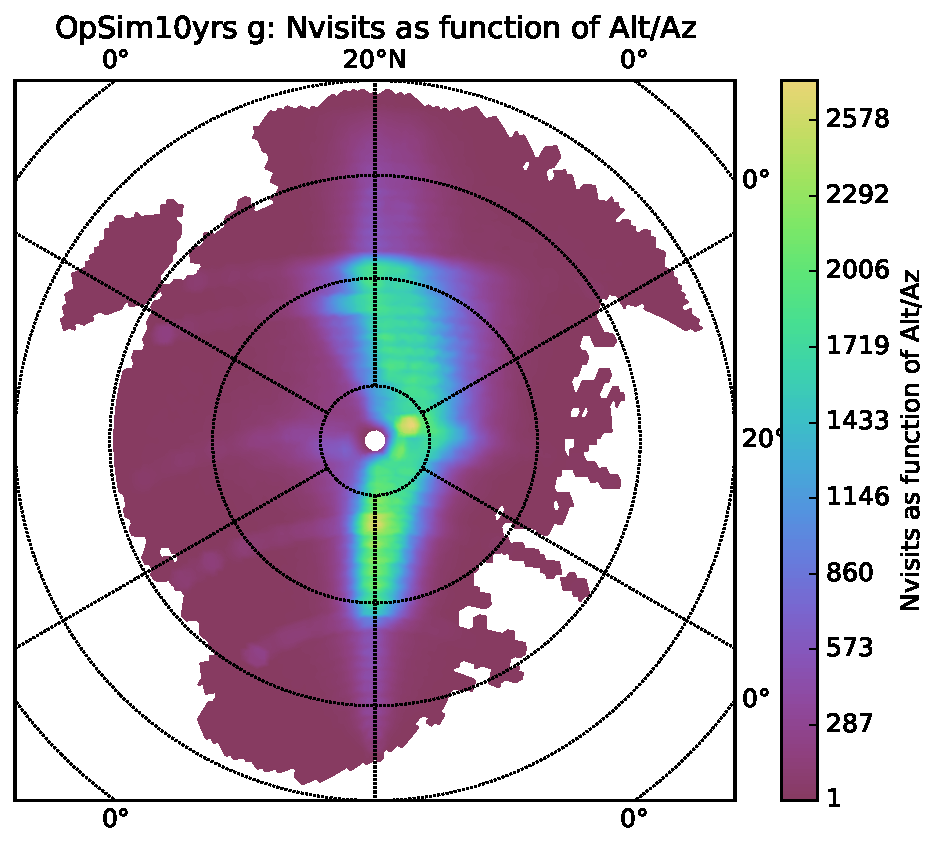
\includegraphics[width=.25\linewidth]{Figures/opsim_Nvisits_as_function_of_Alt_Az_g_HEAL_SkyMap.pdf}&    &  &
%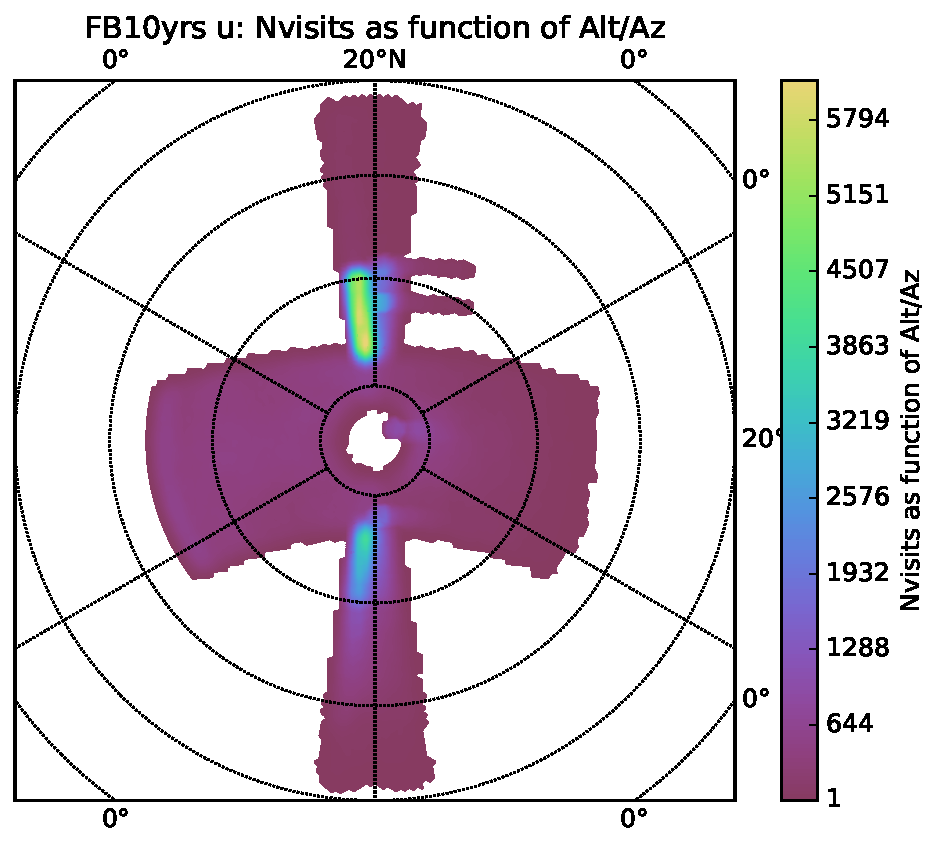
\includegraphics[width=.25\linewidth]{Figures/FB_Nvisits_as_function_of_Alt_Az_u_HEAL_SkyMap.pdf}&
%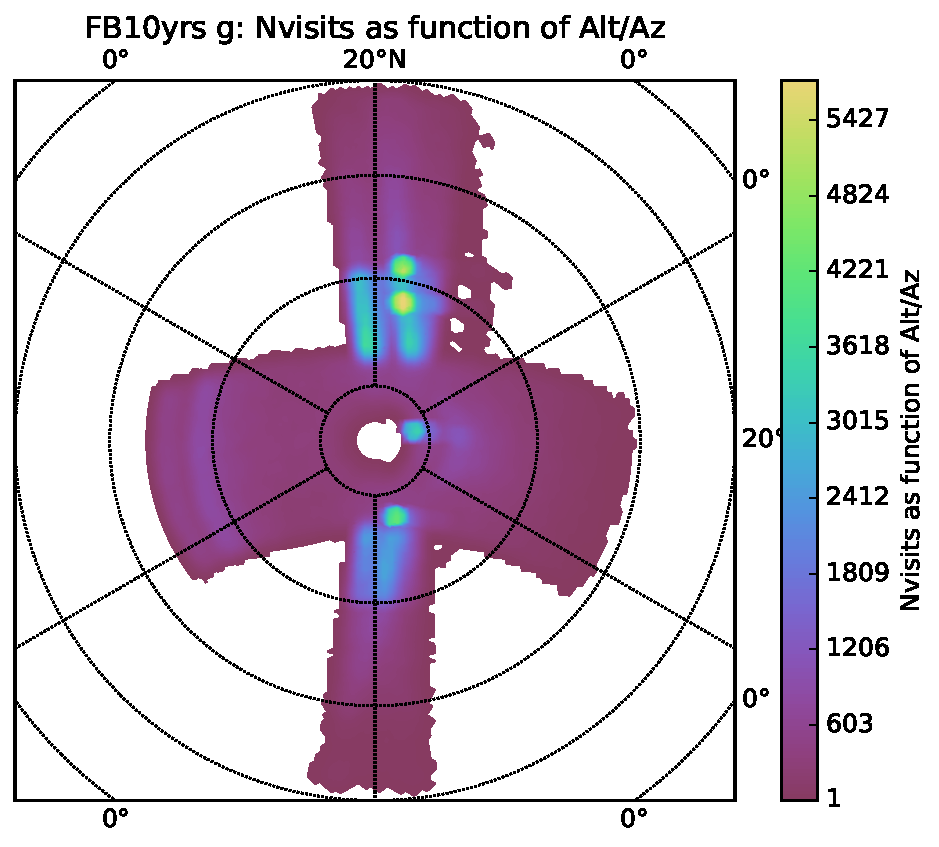
\includegraphics[width=.25\linewidth]{Figures/FB_Nvisits_as_function_of_Alt_Az_g_HEAL_SkyMap.pdf}\\
%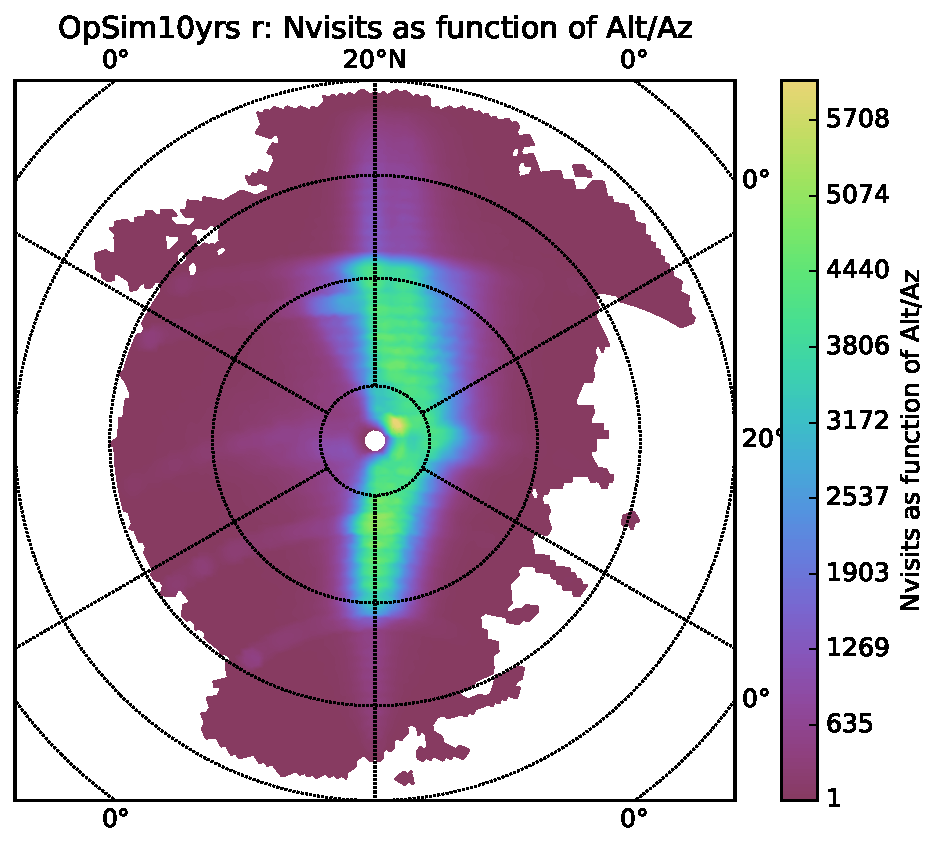
\includegraphics[width=.25\linewidth]{Figures/opsim_Nvisits_as_function_of_Alt_Az_r_HEAL_SkyMap.pdf}&
%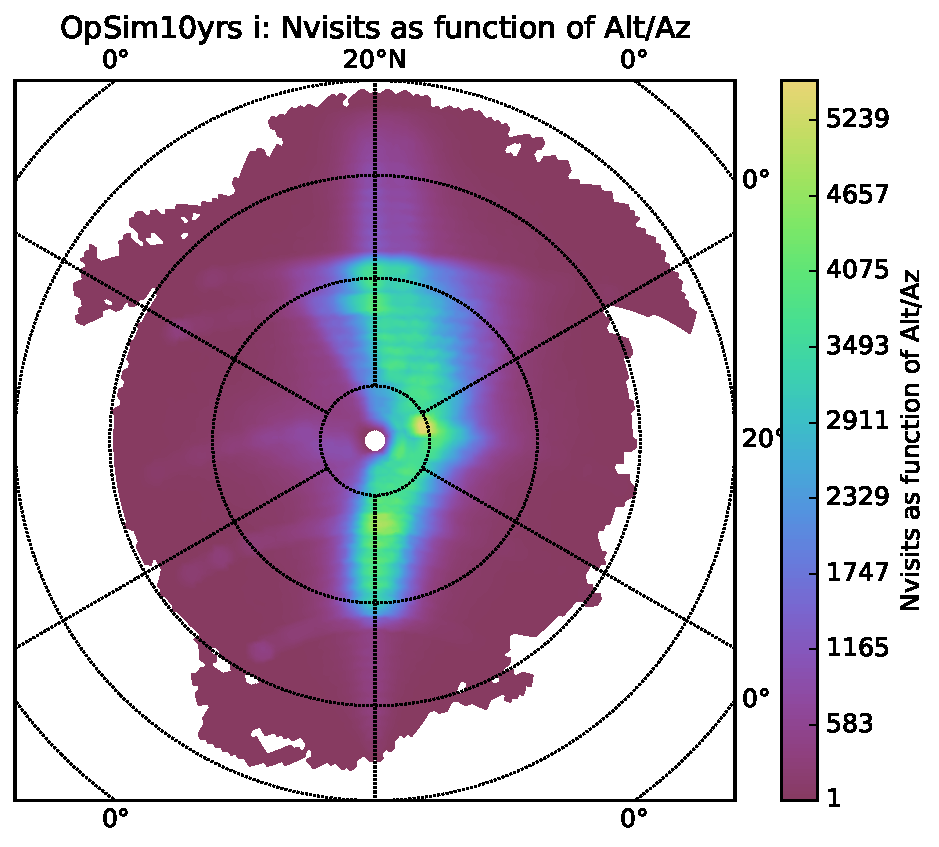
\includegraphics[width=.25\linewidth]{Figures/opsim_Nvisits_as_function_of_Alt_Az_i_HEAL_SkyMap.pdf}&    &  &
%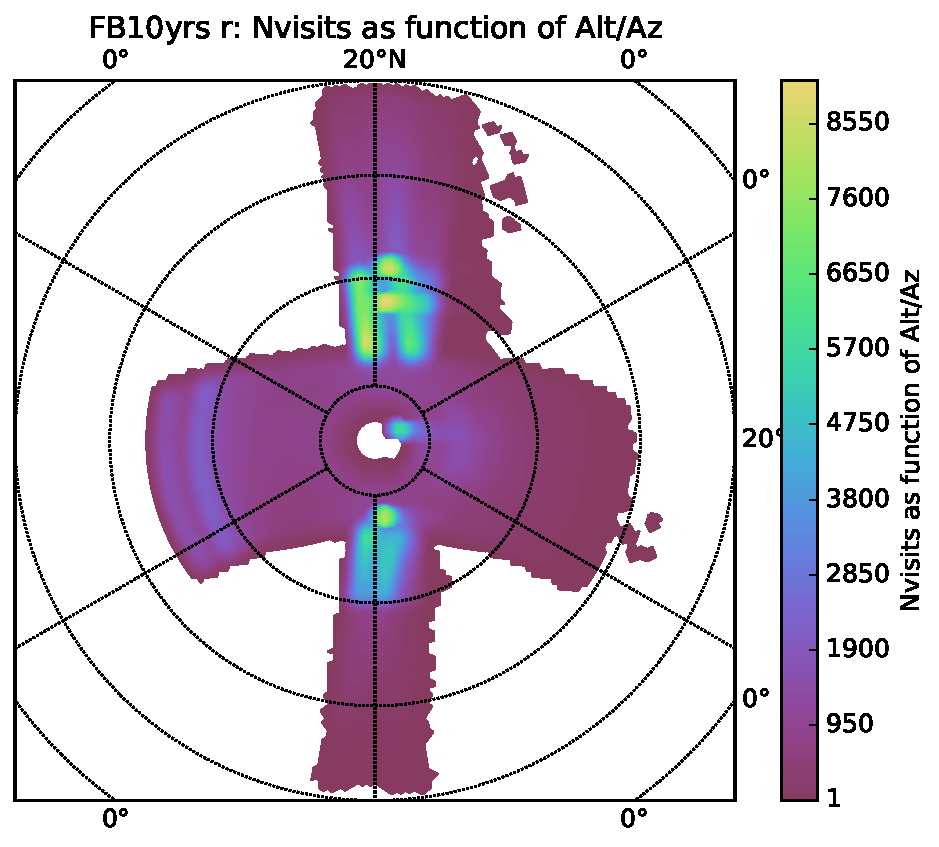
\includegraphics[width=.25\linewidth]{Figures/FB_Nvisits_as_function_of_Alt_Az_r_HEAL_SkyMap.pdf}&
%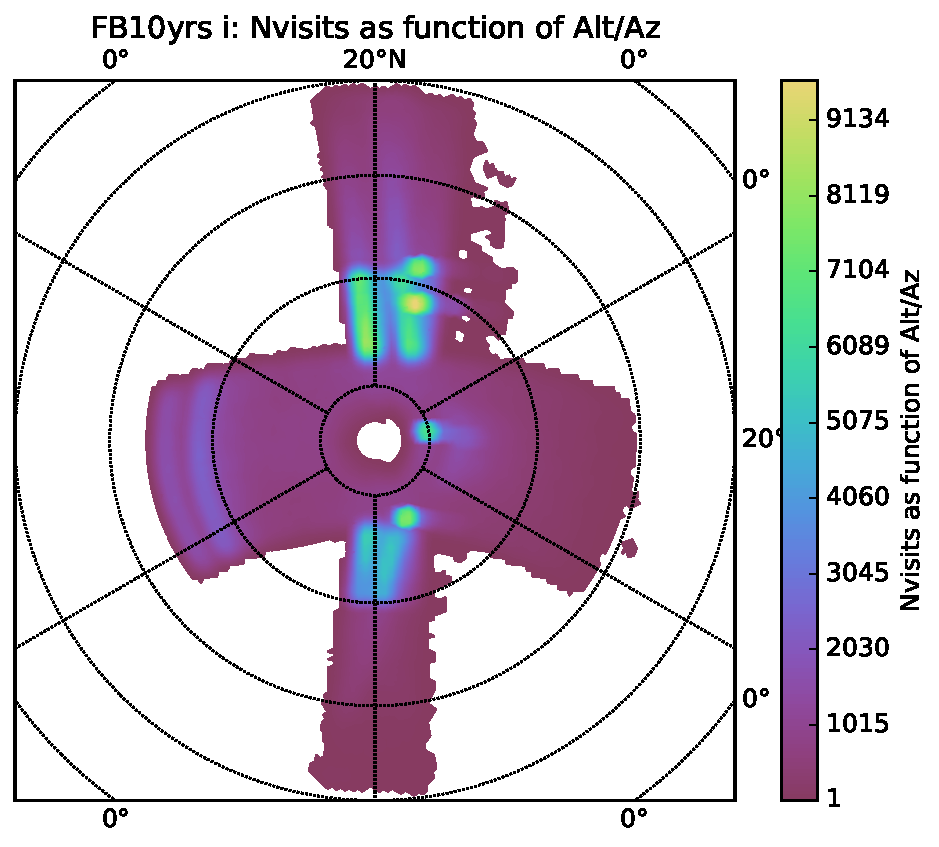
\includegraphics[width=.25\linewidth]{Figures/FB_Nvisits_as_function_of_Alt_Az_i_HEAL_SkyMap.pdf}\\
%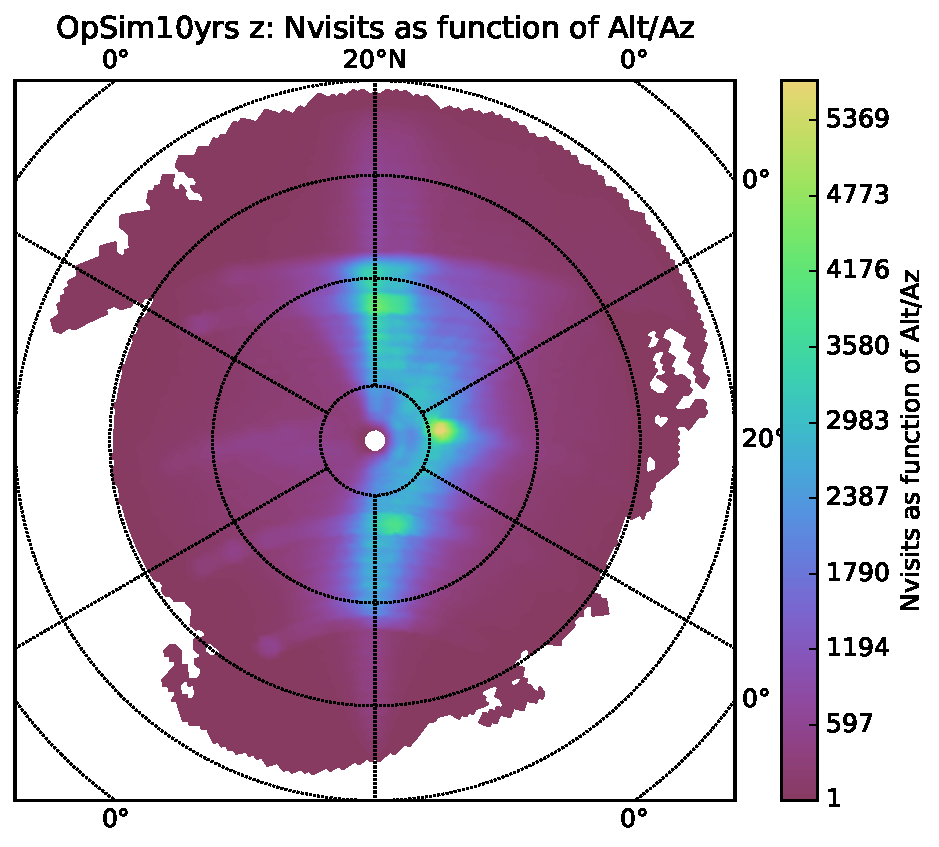
\includegraphics[width=.25\linewidth]{Figures/opsim_Nvisits_as_function_of_Alt_Az_z_HEAL_SkyMap.pdf}&
%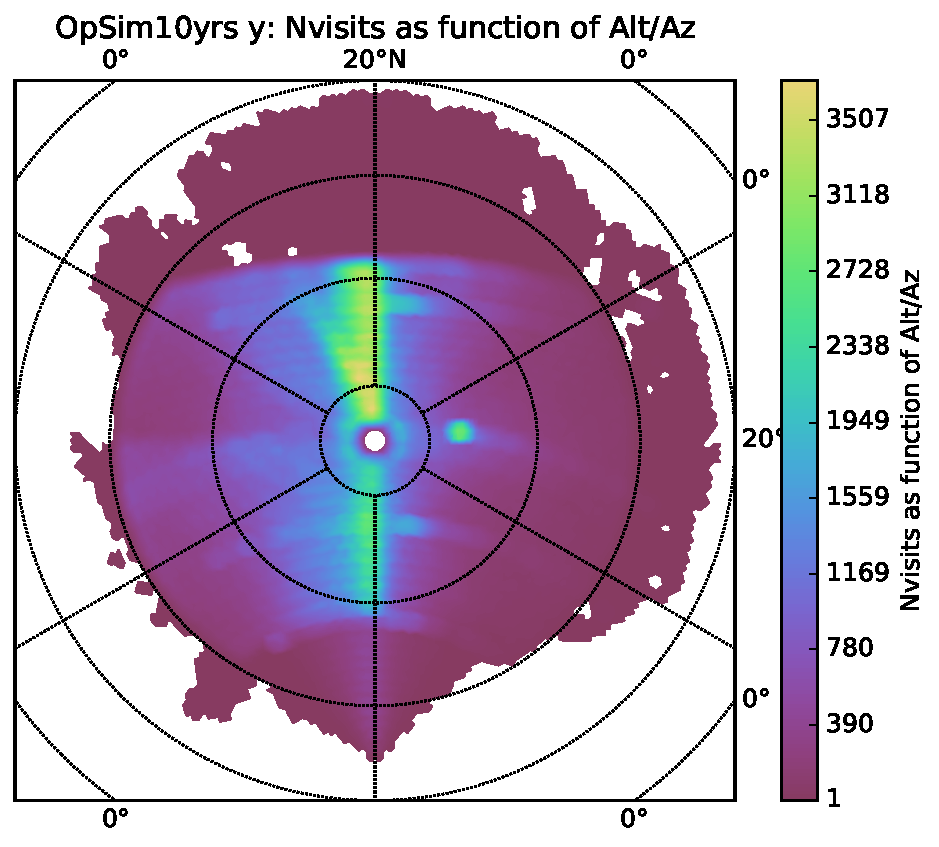
\includegraphics[width=.25\linewidth]{Figures/opsim_Nvisits_as_function_of_Alt_Az_y_HEAL_SkyMap.pdf}&    &  &
%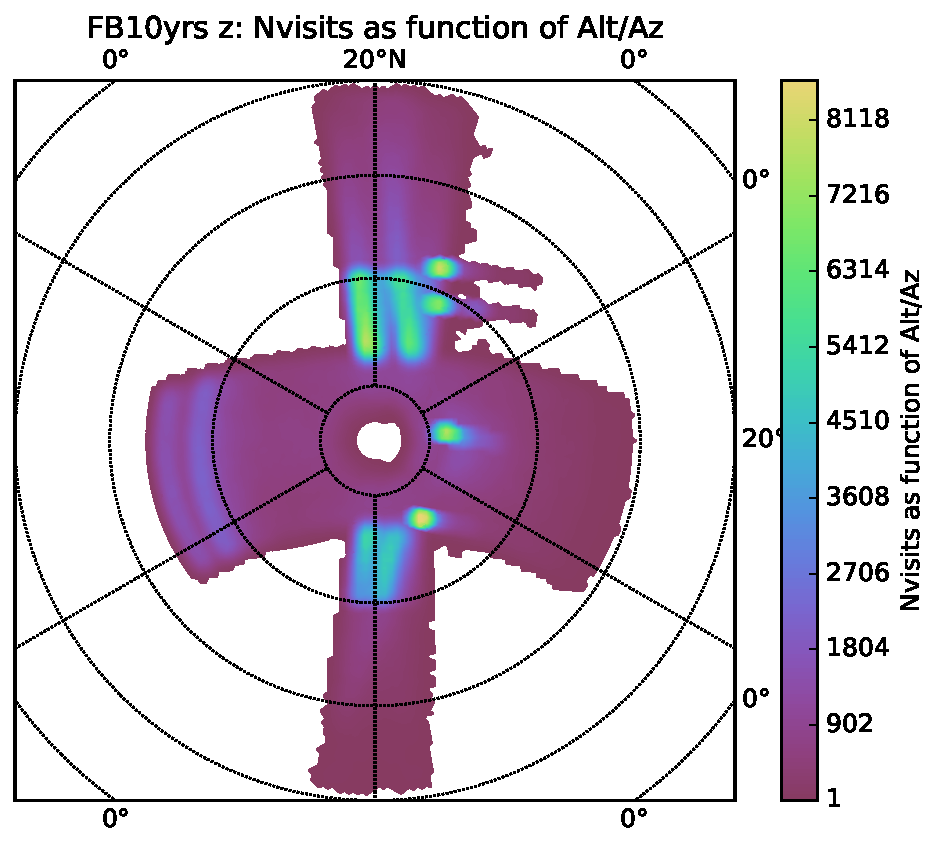
\includegraphics[width=.25\linewidth]{Figures/FB_Nvisits_as_function_of_Alt_Az_z_HEAL_SkyMap.pdf}&
%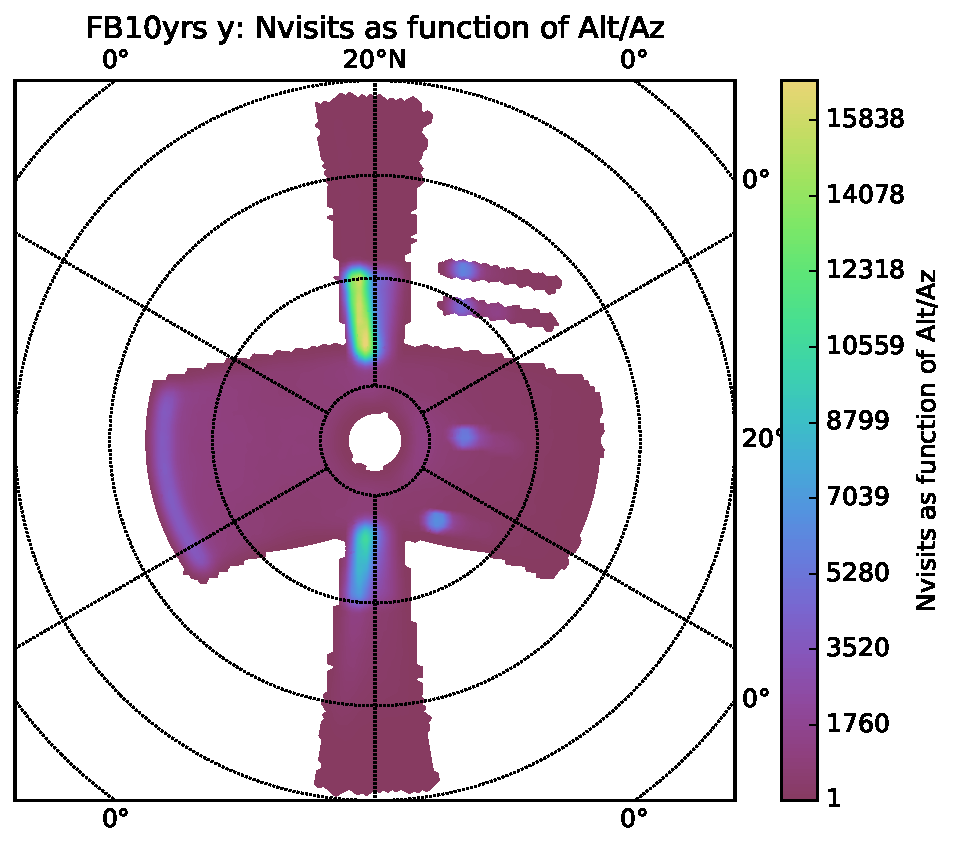
\includegraphics[width=.25\linewidth]{Figures/FB_Nvisits_as_function_of_Alt_Az_y_HEAL_SkyMap.pdf}\\
%\end{array}$
%\end{center}
%\caption{Each plot is the altitude azimuth visit distribution in one of the six filters for 10 years of simulation. The two left columns belong to the \textit{astro-lsst-01-2013} simulation and the two right columns belong to a simulation of the Modified Feature-Based scheduler. The higher concentration on the meridian (vertical axis) for the Modified feature-Based scheduler shows a more desirable behavior. Moreover, consistent concentration of the visits on the east wing can potentially provide a better visit-in-pair behavior}
%\label{fig_10yrs_AltAz}
%\end{figure}
% Figures generated by https://github.com/yoachim/18_scratch/blob/master/bosf_values/BOSF_check.ipynb
\begin{figure}
\begin{center}$
\begin{array}{rcl}
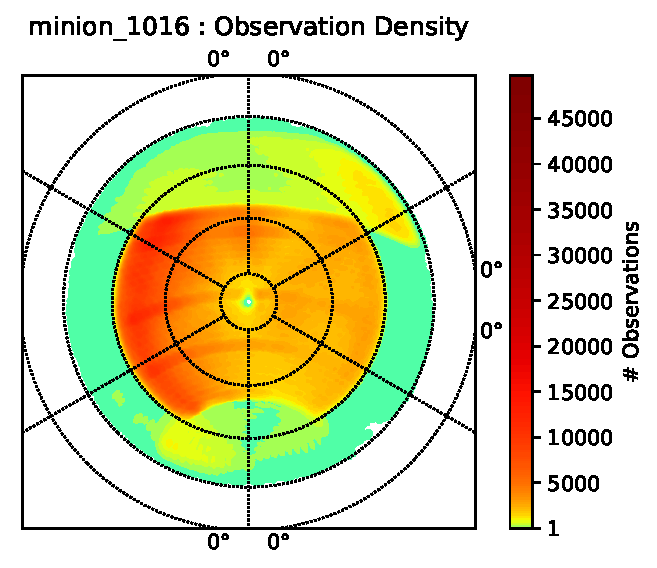
\includegraphics[width = 0.29\textwidth]{Figures/minion_1016_Observation_Density_HEAL_SkyMap.pdf}
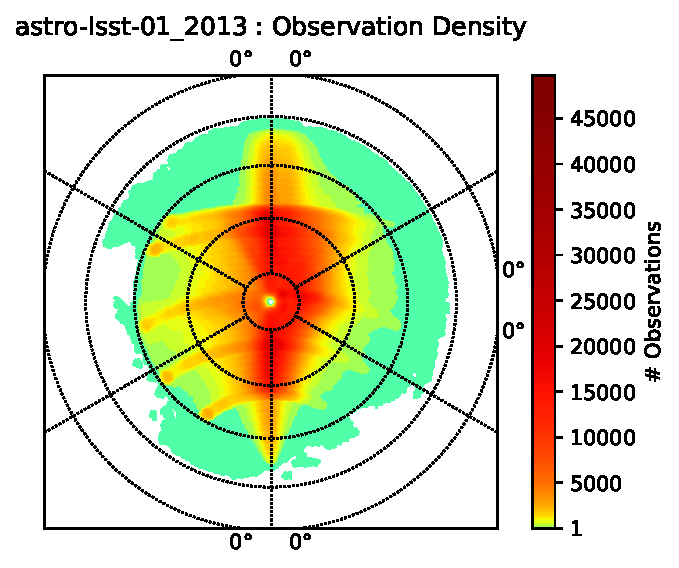
\includegraphics[width = 0.29\textwidth]{Figures/astro-lsst-01_2013_Observation_Density_HEAL_SkyMap.pdf}
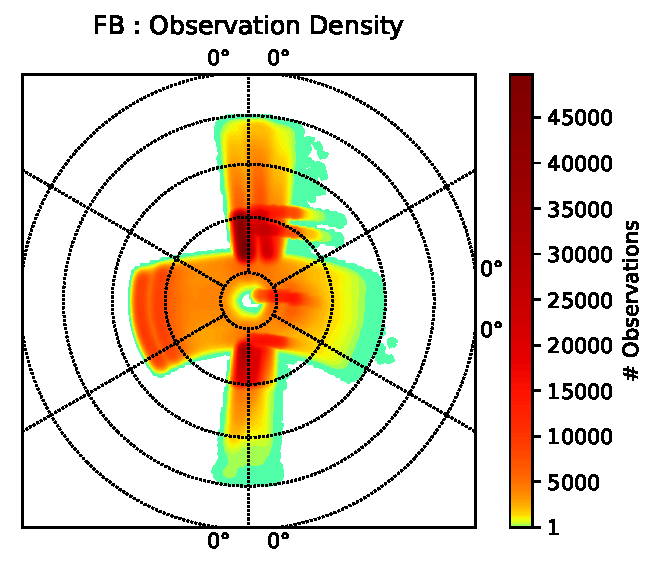
\includegraphics[width = 0.29\textwidth]{Figures/FB_Observation_Density_HEAL_SkyMap.pdf}
\end{array}$
\end{center}
\caption{The altitude azimuth visit distribution for three LSST simulations. On the left, the proposal based minion\_1016 simulation takes most observations at high airmass and very few on the meridian. In the middle, the astro-lsst-01\_2013 simulation takes many observations on the meridian, but still executes deep drilling fields and a smattering of other observations at high airmass. On the right, the feature based simulation concentrates observations, including deep drilling fields, while avoiding observing near zenith. }\label{fig_all_alt_az}
\end{figure}

\section{Concluding remarks}\label{sec_conclusion}
This study demonstrated that a Markovian scheduler based on expert-designed features, and a parametrized decision making policy, can be successfully applied to multi-mission, ground-based telescopes such as LSST. Unlike the mainstream telescope schedulers, Feature-Based scheduler does not rely on hand-crafted observation proposals. Instead, by bringing the decision making process to the individual observation level improves the efficiency of the telescope's operation. In particular, because with this approach the telescope's schedule can be designed for optimality in addition to feasibility, and in general, because schedulers that rely on human interaction are fundamentally prone to potential suboptimality, mainly due to the manual tailoring based on inspections of the instances. Moreover, adjusting their behavior is inconvenient and time consuming in practice. Moreover, being modeled as a Markovian Decision Process, Feature-Based scheduler offers a systematic approach to the optimization of the scheduler's behavior under uncertainties and interruptions.\\
On the other hand, the decision elements in the Feature-Based scheduler are designed, and separated in an intuitive way for the astronomy community that allows for expert intervention if needed, however in a regulated way, and only on the parameters of the policy. Manual adjustments of the parameters of the policy does not break measurability, linearity, and memorylessness of the process. Thus all of the simplicity, optimality conditions and modularity of the design remain valid. In addition, due to the coherent structure, from training to online decision-making, Feature-Based scheduler is easy to understand, implement, and troubleshoot. Simplicity of the design and implementation, also provides a desirable environment for a wide-range of programming expertise in astronomy community to install the python packages on a local computer, define a custom mission objective, train a scheduler and examine the behavior of the scheduler with various mission objectives. Similarly, in a particular project, when a change in the mission's objective is necessary, deriving a new scheduler that optimizes the new objective is principally automated. Furthermore, for the mission planning stage of a future instrument, a scheduler with adjustable objective can be extremely helpful, because it can answer high-level trade-off questions such as the amount of the time efficiency loss in different strategies of capturing transient objects.\\
Furthermore, the required computational resources for the training/optimizing of the Feature-Based scheduler is versatile, depending on the purpose. If many different objective functions are being tested for planning a mission, then a quick $e$DE optimization for a short scheduling episode can find a sufficiently good scheduler for each mission or even a quick manual hand tuning that reflects the intuitive importance of each basis function is possible, because they carry an astronomical observation meaning. On the other hand if the objective is known and fixed, and the scheduler is being trained for real-time decision making, then one might even categorize the observation nights based on their main differences, such as the moon-phase and train a scheduler specifically for each category. 


%\acknowledgments
\textbf{Acknowledgments.} We would like to thank the LSST corporation's leadership for the financial support of this work, and the DIRAC Institute's faculty and researchers for providing expertise, without which this research would not have been possible. In particular, Professor \v{Z}eljko Ivezi\'{c} whose consistent attention and insightful comments greatly assisted this work. We would also like to show our gratitude to the LSST experts in other institutes, specially Professor Michael Strauss, Professor Christopher Stubbs, Dr. Robert Lupton, and Michael Reuter for their insightful comments spanning from the idea stage to the end of this project.
%\facility{LSST}

%\software{MAF \cite{jones2014lsst}, healpy \cite{Healpy05}, matplotlib \cite{matplotlib07}, 
%          astropy \cite{astropy18}, XXX-numpy/scipy}

%\bibliographystyle{unsrt}
\bibliography{/Users/enaghib/Dropbox/Graduate/Research/Princeton/Publications/references}
%\bibliography{references}
\end{document}


